%%%%%%%%%%%%%%%%%%%%%%%%%%%%%%%%%%%%%%%%%%%%%%%%%%%%%%%%%%%%%%%%%%%%
%% I, the copyright holder of this work, release this work into the
%% public domain. This applies worldwide. In some countries this may
%% not be legally possible; if so: I grant anyone the right to use
%% this work for any purpose, without any conditions, unless such
%% conditions are required by law.
%%%%%%%%%%%%%%%%%%%%%%%%%%%%%%%%%%%%%%%%%%%%%%%%%%%%%%%%%%%%%%%%%%%%

\documentclass[
  digital,     %% The `digital` option enables the default options for the
               %% digital version of a document. Replace with `printed`
               %% to enable the default options for the printed version
               %% of your thesis.
%%  color,       %% Uncomment these lines (by removing the %% at the
%%               %% beginning) to use color in the printed version of your
%%               %% document
  oneside,     %% The `oneside` option enables one-sided typesetting,
               %% which is preferred if you are only going to submit a
               %% digital version of your thesis. Replace with `twoside`
               %% for double-sided typesetting if you are planning to
               %% also print your thesis. For double-sided typesetting,
               %% use at least 120 g/m² paper to prevent show-through.
  nosansbold,  %% The `nosansbold` option prevents the use of the
               %% sans-serif type face for bold text. Replace with `sansbold` to use sans-serif type face for bold text.
  nocolorbold, %% The `nocolorbold` option disables the usage of the
               %% blue color for bold text, instead using black. Replace with `colorbold` to use blue for bold text.
  lof,         %% The `lof` option prints the List of Figures. Replace
               %% with `nolof` to hide the List of Figures.
  lot,         %% The `lot` option prints the List of Tables. Replace
               %% with `nolot` to hide the List of Tables.
]{fithesis4}
%% The following section sets up the locales used in the thesis.
\usepackage[resetfonts]{cmap} %% We need to load the T2A font encoding
\usepackage[T1,T2A]{fontenc}  %% to use the Cyrillic fonts with Russian texts.
\usepackage[
  main=english, %% By using `czech` or `slovak` as the main locale
                %% instead of `english`, you can typeset the thesis
                %% in either Czech or Slovak, respectively.
  english, german, czech, slovak %% The additional keys allow
]{babel}        %% foreign texts to be typeset as follows:
%%
%%   \begin{otherlanguage}{german}  ... \end{otherlanguage}
%%   \begin{otherlanguage}{czech}   ... \end{otherlanguage}
%%   \begin{otherlanguage}{slovak}  ... \end{otherlanguage}
%%
%%
%% The following section sets up the metadata of the thesis.
\thesissetup{
    date        = \the\year/\the\month/\the\day,
    university  = mu,
    faculty     = fi,
    type        = mgr,
    department  = ,
    author      = {Bc. Maxmilián Šeffer},
    gender      = m,
    advisor     = {doc. Ing. Václav Oujezský, Ph.D.},
    title       = {Smart Timesheet App},
    TeXtitle    = {Smart Timesheet Application},
    keywords    = {audio transcription, time tracking, mobile application, cloud computing, voice recognition, natural language processing, generative AI, user experience, offline functionality, multilingual support},
    TeXkeywords = {audio transcription, time tracking, mobile application, cloud computing, voice recognition, natural language processing, generative AI, multilingual support, \ldots},
    abstract    = {%
        This thesis explores the potential of audio transcription technology to simplify time tracking for employees working in the field. The goal is to develop a cloud-based application that allows employees to log their working hours by recording audio descriptions of their tasks, specifying the client and project. This recorded speech is then transcribed into text and converted into structured database entries. The research evaluates the reliability and practicality of this approach in real-world conditions.
        
        In addition to automated transcription, the application provides features for replaying audio recordings, manually editing and managing entries, and exporting data for managerial review. By simplifying the logging process, the solution aims to minimize forgetfulness of employees and improve accuracy of work record while offering employees an efficient way to track their work.
    },
    thanks      = {%
      I would like to thank doc. Ing. Václav Oujezský, Ph.D., for his guidance and leadership throughout this thesis. My thanks also go to Bc. Ondřej Zelinka, with whom I collaborated as he was working simultaneously on a web version of the front-end. I am also grateful to Roman Kalous for his support and cooperation on behalf of the company.
    },
    bib         = example.bib,
    %% Remove the following line to use the JVS 2018 faculty logo.
    facultyLogo = fithesis-fi,
}
\usepackage{makeidx}      %% The `makeidx` package contains
\makeindex                %% helper commands for index typesetting.
%% These additional packages are used within the document:
\usepackage{paralist} %% Compact list environments
\usepackage{amsmath}  %% Mathematics
\usepackage{amsthm}
\usepackage{amsfonts}
\usepackage{url}      %% Hyperlinks
\usepackage{markdown} %% Lightweight markup
\usepackage{listings} %% Source code highlighting
\usepackage{xcolor}
\lstdefinelanguage{Dart}{
  keywords={
    abstract, as, assert, async, await, break, case, catch, class, const, continue,
    covariant, default, deferred, do, dynamic, else, enum, export, extends, extension,
    external, factory, false, final, finally, for, Function, get, hide, if, implements,
    import, in, interface, is, late, library, mixin, new, null, on, operator, part,
    required, rethrow, return, set, show, static, super, switch, sync, this, throw,
    true, try, typedef, var, void, while, with, yield
  },
  keywords=[2]{@override, @JsonSerializable, @deprecated, @protected, @required, @visibleForTesting}, % Group 2: annotations
  sensitive=true,
  comment=[l]{//},
  morecomment=[s]{/*}{*/},
  morestring=[b]",
  morestring=[b]',
}
\lstset{
  basicstyle      = \ttfamily,  % <-- monospace
  identifierstyle = \color{black},
  keywordstyle    = \color{blue}\bfseries,
  keywordstyle=[2]\color{orange}\bfseries,
  stringstyle     = \color{teal},
  commentstyle    = \itshape\color{magenta},
  breaklines      = true,
  columns         = flexible,          % <-- no weird spacing
  keepspaces      = true,               % <-- keep spacing in code
  showstringspaces= false,              % <-- hide weird markers in spaces
}
\usepackage{floatrow} %% Putting captions above tables
\usepackage{pgfplots}
\pgfplotsset{compat=1.18}
\floatsetup[table]{capposition=top}
\usepackage[babel]{csquotes} %% Context-sensitive quotation marks

\begin{document}
%% The \chapter* command can be used to produce unnumbered chapters:
\chapter*{Introduction}
%% Unlike \chapter, \chapter* does not update the headings and does not
%% enter the chapter to the table of contents. If we want correct
%% headings and a table of contents entry, we must add them manually:
\markright{\textsc{Introduction}}
\addcontentsline{toc}{chapter}{Introduction}
TODO

\begin{otherlanguage}{czech}
TODO
\end{otherlanguage}

\chapter{System Requirements}

\section{Introduction}

In order to develop a practical and effective cloud-based audio transcription system for time tracking, a comprehensive requirements analysis is essential. This phase establishes a clear understanding of the functionalities and constraints that the software must adhere to, ensuring alignment with user needs and business objectives. The analysis focuses on defining user roles, identifying functional and non-functional requirements, and outlining key technical considerations.

The goal of this analysis is to create a structured framework that guides the development of the Smart Timesheet Application. Through discussions with potential users, stakeholders, and domain experts, the analysis highlights both explicit and implicit needs, as well as potential challenges that may arise during implementation.

\section{Users}

The primary users of the Smart Timesheet Application are mainly field employees. These users frequently switch between tasks and clients throughout the day. Their primary need is a quick, reliable, and intuitive method to log their working hours and task details in real-time without requiring a traditional computer interface. They benefit from hands-free audio logging that ensures accuracy and minimizes forgotten details.

\section{Functional Requirements}

The functional requirements define the core capabilities of the Smart Timesheet Application, ensuring that it meets user expectations and performs its intended tasks efficiently. These requirements specify the system's behavior in terms of services, tasks, and functions that users can perform.

This section also integrates the functional requirements as outlined by the development team at Devbalance. These include support for multiple languages, offline functionality, voice-to-text processing, and generative AI for text analysis. The integration of these elements helps ensure the application’s performance aligns with the needs of its users while supporting real-time synchronization, data accuracy, and ease of use.

To clearly outline the expected functionality, the requirements are presented in the form of use cases. Each use case describes a specific interaction between the user and the system, defining the prerequisites, the sequence of steps, and the expected outcome.

The use cases are not listed by priority but instead grouped at the same level of abstraction for clarity. While some use cases could be decomposed into more detailed subcases, this document keeps them at a high level to maintain readability. Detailed business logic, rules, and dependencies will be enforced through integration tests in the system’s codebase, avoiding redundant specifications in this document.

The core functional requirements of the Smart Timesheet Application revolve around efficient, voice-enabled time tracking, cloud-based data storage, secure authentication, and multi-language support. The application must accommodate hands-free logging while ensuring that users can review, edit, and manage their work records with minimal friction. Additionally, robust data security mechanisms must be in place to guarantee data integrity and user privacy. The system should also provide offline and online synchronization, as well as support for generative AI to analyze and summarize work entries.

\subsection{Voice-to-Text Recording and Storage}

\noindent \textbf{Actors:} Employee

\noindent \textbf{Prerequisites:} User is authenticated

\noindent \textbf{Description:}  
Employees can record audio descriptions of their work in either Czech or English. The system transcribes the audio into text, uses a trained AI model to extract key information, and stores the recording in a cloud-based NoSQL database. The extracted data is parsed into a structured database entry, first saved locally and then persistently in the cloud.

\noindent \textbf{Steps:}
\begin{enumerate}
    \item Employee initiates an audio recording in the application.
    \item Employee verbally describes the work performed, using either Czech or English.
    \item The system automatically detects the language of the recording if not manually selected.
    \item System uploads the recording to the cloud.
    \item Transcription service processes the audio and converts it into text.
    \item AI model analyzes the transcribed text, extracting key information such as client, task, activity, and duration.
    \item System structures the extracted data into a work record.
    \item Work record is temporarily saved locally on the device.
    \item Work record is uploaded to the cloud-based NoSQL database.
    \item The employee receives a notification upon completion of the transcription and data entry.
\end{enumerate}

\subsection{Adding Work Records Manually}

\noindent \textbf{Actors:} Employee

\noindent \textbf{Prerequisites:} User is authenticated

\noindent \textbf{Description:}  
Employees can manually enter work records if they prefer not to use audio transcription or if they wish to edit a previously recorded work entry.

\noindent \textbf{Steps:}
\begin{enumerate}
    \item Employee navigates to the manual work entry interface.
    \item Employee inputs details such as client, project, and task description.
    \item Work entry is saved to the cloud database.
\end{enumerate}

\subsection{Reviewing and Editing Work Entries}

\noindent \textbf{Actors:} Employee

\noindent \textbf{Prerequisites:} User is authenticated, work entries exist

\noindent \textbf{Description:}  
Employees can review and edit their past work records, including both manually entered and transcribed entries.

\noindent \textbf{Steps:}
\begin{enumerate}
    \item Employee accesses the work log history.
    \item Employee selects a work entry to review.
    \item Employee can replay the original audio recording (if available).
    \item If necessary, employee edits the transcription or manually entered details.
    \item Updated entry is saved to the cloud database.
\end{enumerate}

\subsection{Searching, Filtering, and Sorting Work Entries}

\noindent \textbf{Actors:} Employee

\noindent \textbf{Prerequisites:} User is authenticated, work entries exist

\noindent \textbf{Description:}  
Employees can search for and filter work logs based on specific criteria such as date, project, or client. Sorting of records is also available.

\noindent \textbf{Steps:}
\begin{enumerate}
    \item Employee accesses the search and filter interface.
    \item Employee selects criteria for filtering (e.g., date range, client, project).
    \item Employee selects criteria for sorting (e.g., by date, project, or client).
    \item System retrieves and displays the matching work entries.
\end{enumerate}

\subsection{Cloud-Based Data Storage and Organization}

\noindent \textbf{Actors:} System

\noindent \textbf{Prerequisites:} Work entries exist

\noindent \textbf{Description:}  
Work records are securely stored in a cloud-based NoSQL database. Employees can access their records from any authenticated device.

\noindent \textbf{Steps:}
\begin{enumerate}
    \item Work entries are saved in a structured format in the cloud.
    \item System ensures data is organized for efficient retrieval.
    \item Employees can easily view, sort, and access their stored records.
\end{enumerate}

\subsection{User Authentication and Access Control}

\noindent \textbf{Actors:} Employee

\noindent \textbf{Prerequisites:} None

\noindent \textbf{Description:}  
Authentication and access control ensure that only authorized users can log in and access their respective data.

\noindent \textbf{Steps:}
\begin{enumerate}
    \item Employee attempts to log in via Microsoft authentication.
    \item System verifies credentials through Firebase Authentication.
    \item System checks the employee’s email domain.
    \item If the domain is authorized, the employee is granted access to their records.
    \item System ensures that employees from different domains cannot view or modify each other's records.
\end{enumerate}

\subsection{Offline Audio Logging and Synchronization}

\noindent \textbf{Actors:} Employee

\noindent \textbf{Prerequisites:} User is authenticated, no internet connection available

\noindent \textbf{Description:}  
Employees can record work descriptions offline. Once an internet connection is restored, the system automatically uploads and processes the recordings, ensuring that data is synchronized across devices.

\noindent \textbf{Steps:}
\begin{enumerate}
    \item Employee records an audio entry while offline.
    \item System stores the recording locally on the device.
    \item Once an internet connection is restored, the system automatically uploads and processes the recording.
    \item Transcribed entry is added to the work log.
\end{enumerate}

\subsection{Receiving Notifications}

\noindent \textbf{Actors:} Employee

\noindent \textbf{Prerequisites:} User is authenticated, relevant event occurs

\noindent \textbf{Description:}  
Employees receive notifications when important events occur, such as transcription completion or record updates.

\noindent \textbf{Steps:}
\begin{enumerate}
    \item System detects an event requiring a notification (e.g., transcription complete).
    \item System generates a notification message.
    \item Employee receives a push notification or email alert.
\end{enumerate}

\subsection{Multilingual User Interface}

\noindent \textbf{Actors:} Employee

\noindent \textbf{Prerequisites:} User is authenticated

\noindent \textbf{Description:}  
Employees can switch between Czech and English for the user interface, allowing the application to support a multilingual user base.

\noindent \textbf{Steps:}
\begin{enumerate}
    \item Employee navigates to the settings menu.
    \item Employee selects the preferred language (Czech or English).
    \item The user interface updates to the selected language.
\end{enumerate}

\section{Non-Functional Requirements}

While functional requirements define what the system must do, non-functional requirements ensure that the system operates effectively under real-world conditions. These requirements specify qualities such as performance, security, usability, and scalability, ensuring that the application remains reliable, efficient, and user-friendly over time.  

The Smart Timesheet Application is designed to accommodate employees working in various environments, including fieldwork where hands-free operation and offline functionality may be necessary. Additionally, as a cloud-based solution, the system must provide seamless data synchronization and high availability, while ensuring that sensitive work records remain secure and private.  

The following sections outline the essential characteristics that the system must meet to provide a smooth, secure, and scalable experience.

\subsection{Performance and Reliability}  
The transcription process does not need to be instant, but users must be notified upon completion so they can review and verify the results. The system must handle multiple concurrent users and organizations without performance degradation.  

While a constant internet connection is not required, users must be able to record audio offline. The recorded audio should be queued and automatically processed when the device reconnects to the internet. Additionally, the system should ensure that no data is lost in case of connection interruptions.

\subsection{Usability and Accessibility}  
The user interface should be designed with simplicity and ease of use in mind, requiring minimal training. Hands-free operation should be a priority, with voice commands and simple touch interactions allowing users to log work efficiently without needing extensive manual input.  

The system should also provide clear visual and auditory feedback to confirm actions. Text should be minimized for core functionality but available for advanced configurations and settings.

\subsection{Security and Compliance}  
All user data must be securely stored and transmitted using encryption. The application must comply with GDPR and other relevant data protection regulations, ensuring that users’ personal and work-related information is not exposed or misused.  

Additionally, access control mechanisms must prevent unauthorized users from accessing or modifying work records.

\subsection{Scalability}  
The system must be designed to support a growing number of users and organizations. As adoption increases, performance should remain stable, and the backend infrastructure must be capable of handling increased storage and processing demands without requiring significant downtime or maintenance.

\subsection{Cross-Platform Support}  
The application must be available on both Android and iOS platforms, ensuring that employees can access and use the system regardless of their device. The mobile application should maintain consistent functionality and usability across different devices and operating system versions.

\subsection{Logging and Audit Trails}  
The system must maintain detailed audit logs for key operations, including the creation and modification of work records. Specifically, changes to work entries, authentication events, and offline-to-online data synchronization must be logged.  

These logs should provide administrators and developers with insights into potential issues, user errors, or security concerns.

\subsection{Failure Handling and Reporting}  
The application must include mechanisms for detecting and reporting failures. If an entry fails to synchronize due to network issues or a transcription error, the user must be notified, and the failure must be logged for further debugging.  

Complete system failures should be automatically reported to the development team, enabling proactive maintenance and issue resolution.

\subsection{Database Support}  
The system should efficiently handle up to a million records and a million audio files without performance degradation.  

\subsection{Performance Optimization}  
The system must be optimized for fast data loading and processing, even with large volumes of records. Voice recordings should be quickly accessible for playback, ensuring a responsive user experience.

\subsection{Storage Capacity}  
The system must efficiently manage storage for millions of short voice files of medium quality. It should automatically optimize storage usage while ensuring quick access to the files when needed.

\subsection{Voice Recordings Security}  
Voice recordings must be securely encrypted both during transmission and at rest. The system should ensure that sensitive voice data remains protected from unauthorized access or tampering.

\subsection{Multilingual Support}  
The application must support two language variants (Czech and English) for the user interface and for processing text from voice recordings. This includes ensuring that the transcription, AI models, and interface components can handle both languages seamlessly.

\subsection{Testability and Logging}  
The system must include detailed logging of user actions and error reports that facilitate testing and debugging. Logs should capture important events such as the creation and modification of records, authentication attempts, and synchronization statuses.

\subsection{Data Backup}  
The system must support automatic backup of both structured data and voice recordings on a regular basis. This ensures data integrity and recovery in case of system failures or data loss events.

\subsection{UI Responsiveness}  
The user interface must be responsive and provide a consistent user experience across devices, including smartphones, tablets, and desktops. The application should adapt seamlessly to different screen sizes and resolutions to ensure usability in both small and large devices.

    
\shorthandoff{-}
\begin{markdown}[
  citationNbsps,
  citations,
  definitionLists,
  fencedCode,
  hashEnumerators,
  inlineNotes,
  notes,
  pipeTables,
  rawAttribute,
  tableCaptions,
]
   
\end{markdown}
\shorthandon{-}

\chapter{Market Analysis}

\section{Introduction}
The need for efficient time-tracking solutions has led to the development of various tools aimed at helping businesses and employees manage work hours effectively. Many existing solutions rely on manual entry, mobile applications, or automated tracking features. However, there are still gaps in usability, accuracy, and hands-free operation, particularly for field employees who require a more seamless and automated way to log their time.

\section{Existing Solutions}

Several time-tracking applications currently serve businesses, each with strengths and limitations:

\begin{itemize}
\item \textbf{Clockify}: A widely used time-tracking tool that provides manual entry, timers, and integration with various project management tools. While powerful, it requires manual input or interaction with a timer, which may not be ideal for field employees who need a hands-free option.
\item \textbf{Toggl Track}: Offers intuitive time tracking with automation features, but still relies on user interaction to start and stop time logs. It lacks built-in voice transcription for work entry.
\item \textbf{Hubstaff}: Includes GPS tracking and automated timesheets, making it useful for remote teams, but does not focus on voice-based logging.
\item \textbf{TSheets by QuickBooks}: Provides detailed time-tracking features and payroll integration but requires manual input or GPS tracking, with no emphasis on voice-based automation.
\end{itemize}

\section{Strengths and weaknesses of existing solutions}

\begin{itemize}  
    \item \textbf{Strengths:} Most existing solutions provide cloud-based tracking, integrations with payroll and project management tools, and mobile accessibility. In addition, these applications are often highly optimized and feature rich, ensuring a streamlined user experience. However, many of their most valuable features are restricted behind paywalls, necessitating costly subscriptions. Moreover, businesses frequently lack control over the application's functionality and long-term availability, making them dependent on third-party providers. Organizations require a time-tracking solution that offers reliability and stability without the risk of unexpected feature limitations, forced upgrades, or service discontinuation.  

    Another significant limitation is the absence of dedicated audio-to-work-entry functionality in existing solutions. Although some applications permit audio attachments as supplementary notes, they do not provide automated transcription or structured conversion of voice recordings into work entries. As a result, users must rely on manual data entry or timers, which may be inefficient for field employees who require a seamless and hands-free method of logging work hours.  

    \item \textbf{Weaknesses:} The majority of existing solutions rely on manual input, timers, or GPS tracking, which may be impractical for employees working in dynamic field environments. Although some applications incorporate voice-based logging, these implementations are generally limited to note taking rather than full transcription and structured work entry generation. Consequently, such solutions function more as auxiliary documentation tools rather than complete work-logging systems, failing to address the specific needs of professionals who require accurate and automated time tracking.

\end{itemize}

\shorthandoff{-}
\begin{markdown}[
  citationNbsps,
  citations,
  definitionLists,
  fencedCode,
  hashEnumerators,
  inlineNotes,
  notes,
  pipeTables,
  rawAttribute,
  tableCaptions,
]
\end{markdown}
\shorthandon{-}


\shorthandoff{-}
\begin{markdown}[
  citationNbsps,
  citations,
  definitionLists,
  fencedCode,
  hashEnumerators,
  inlineNotes,
  notes,
  pipeTables,
  rawAttribute,
  tableCaptions,
]

# Design

## Overview

The Smart Timesheet Application is designed to provide a scalable and efficient solution for employees to log and manage their work records using audio-based logging and manual entry. The system must handle multiple companies, ensuring that user authentication, data storage, and processing are both secure and scalable.

A fundamental design decision was to offload authentication and user management to Microsoft accounts. Since the application is expected to be used across different companies, managing user accounts internally would introduce unnecessary complexity. By leveraging Microsoft's identity management services, authentication and access control are handled externally, ensuring a seamless and secure login experience while eliminating the need for manual account management.

The backend of the system is entirely cloud-based, ensuring high availability, real-time synchronization, and scalability. A NoSQL cloud database stores all timesheet entries, while audio recordings are uploaded to cloud storage, making them accessible from both mobile and web applications. Various approaches were considered, including self-hosted database solutions such as MongoDB or SQLite with a shared repository layer. While these could provide flexibility in local or hybrid deployments, they introduce challenges such as scalability limitations, synchronization complexity, and increased maintenance overhead. A cloud-first approach was chosen to provide automatic scaling, seamless access across devices, and minimal operational burden.

A key feature of the application is converting audio logs into structured timesheet entries. This is achieved through external Open API endpoints that handle both speech-to-text transcription and text-to-timesheet parsing. Running a lightweight AI model directly on mobile devices was considered as an alternative, but this approach was ultimately discarded due to performance constraints, high battery consumption, difficulty in maintaining AI models across different devices, and inconsistent processing power across smartphones. By utilizing cloud-based AI services, the system ensures accurate and scalable transcription without compromising device performance.

The primary interface for users is a mobile application, available for both Android and iOS. The mobile app allows employees to record audio logs, manually enter work records, and review their timesheet history. The user experience is designed to be minimalistic and intuitive, prioritizing voice-based interactions and quick data entry.

In addition to the mobile app, there is also a web-based application, which provides an alternative way for users to access their timesheet data. The web application was developed independently by Bc. Ondřej Zelinka as a separate implementation. However, since both applications were meant to be interchangeable from the view of the user, the design and core functionalities of the entire system were discussed before and through their implementation, then aligned to ensure consistency between platforms. While both applications were implemented separately, they share many technical details related to backend services, including transcription models, prompts, database structures, and user group management. This ensures that both platforms provide a unified experience and operate on the same fundamental principles.

In conclusion, the system was designed with a strong emphasis on improving user experience, scalability, and operational efficiency. By utilizing Microsoft accounts for authentication, the application ensures secure and simplified access management, particularly important given the multi-organization use case. Cloud-based storage for data and audio recordings guarantees high availability, scalability, and seamless real-time synchronization across devices. The integration of external AI services for transcription offloads resource-intensive processing to a third party, reducing system complexity without introducing a critical backend service that would require additional maintenance and most importantly, availability management.

\end{markdown}

\section{System Architecture}

The system architecture is designed with a clear focus on scalability, efficiency, and cross-platform functionality. After careful consideration of the system requirements, along with some prototyping, it has been decided that the core functionality will be supported by the following components.

The development process has been conducted concurrently a mobile and a web interface\footnote{The web application is not a part of this thesis and has been developed by a fellow student, Bc. Ondřej Zelinka}. Although developed as separate projects, they share many common features and functionalities. Notably, the UI/UX designs have been discussed and aligned across both platforms. A shared set of supporting services ensures that both the mobile app and the web interface operate seamlessly, offering a consistent experience. These shared services include the entire Firebase stack, which provides authentication, data storage, and standardization of timesheet data formats. Furthermore, the OpenAI endpoints and associated prompts are employed as common resources for both applications and saved in Firebase storage. This design allows the user to utilize both applications simultaneously with a single account, ensuring a unified experience across platforms.

\subsection{System Components Overview}

The core components of the system include:

\begin{itemize}
    \item \textbf{Android/iOS Application} – A mobile application available on both Android and iOS platforms, providing users with access to the system's functionalities.
    \item \textbf{Web Application} – Developed by a fellow student, Bc. Ondřej Zelinka, as a separate project. This web-based platform offers similar functionalities to the mobile application, allowing users to interact with the system via a web browser.
    \item \textbf{OpenAI API}
    \begin{itemize}
        \item \textbf{Speech-to-Text Endpoint} – Used for transcribing audio recordings to text.
        \item \textbf{Text-to-Timesheet Endpoint} – Converts the transcribed text into a structured timesheet format.
    \end{itemize}
    \item \textbf{Firebase Services}
    \begin{itemize}
        \item \textbf{Firebase Storage} – Used for storing audio files.
        \item \textbf{Firestore Database} – A NoSQL database used to store static content such as prompts, activities, clients, and projects, as well as dynamic data such as timesheets.
        \item \textbf{Firebase Authentication} – A service used for managing user authentication across both platforms.
    \end{itemize}
    \item \textbf{Azure App} – Provides finer control over login procedures via Microsoft accounts, as this is the primary method of authentication, as required by Devbalance.
\end{itemize}

Several additional services and supporting components are used and further discussed in the Deployment chapter. 

\shorthandon{-}

\chapter{Technologies used}

The Smart Timesheet Application is built using modern technologies that ensure scalability, performance, and security. The choice of technologies directly supports the functional and non-functional requirements, enabling efficient development and a seamless user experience. The key technologies used in the application include Flutter, Firebase, and Microsoft Authentication.

\section{Flutter}

Flutter is a UI framework developed by Google that allows for the development of natively compiled applications for mobile, web, and desktop from a single codebase. The Smart Timesheet Application uses Flutter to create cross-platform applications for both Android and iOS devices.

Flutter utilizes the Dart programming language, which offers a rich set of features and provides strong typing, asynchronous programming, and fast performance. By using Flutter, the application is able to maintain consistent functionality and high performance across different platforms.

The core advantage of Flutter lies in its hot reload feature, which allows developers to instantly see changes in the code reflected in the application without needing to restart the app. This significantly speeds up development time and improves the testing cycle.

\section{Firebase}

Firebase is a comprehensive platform for building web and mobile applications, offered by Google. It provides a set of tools that simplifies backend development, handling key tasks such as data storage, authentication, and crash reporting.

\subsection{Firestore}

Firestore is a NoSQL cloud database that is used in the Smart Timesheet Application to store work records and user data. Firestore allows for scalable and flexible storage, offering real-time synchronization of data across all devices. This is crucial for ensuring that the data is always up-to-date across different devices, especially when working offline or in poor network conditions.

Data in Firestore is stored in collections of documents. Each document contains fields, where data is stored as key-value pairs. This structure allows easy querying and retrieval of user data, making it suitable for the dynamic nature of the application.

\subsection{Firebase Storage}

Firebase Storage is used for storing and serving large files, such as voice recordings. The Smart Timesheet Application uses Firebase Storage to securely store audio files that users upload as part of their work records. The integration of Firebase Storage ensures that these files are available for download and playback in a fast and secure manner.

\subsection{Crashlytics}

Firebase Crashlytics is a powerful crash reporting tool integrated into the Smart Timesheet Application to track, report, and fix crashes in real-time. Crashlytics provides detailed reports about the nature and frequency of crashes, allowing developers to quickly identify and resolve critical issues, improving the app's stability.

\subsection{Firebase Authentication}

Firebase Authentication is used to manage user sign-in and authentication within the application. The Smart Timesheet Application utilizes Microsoft authentication to allow users to sign in securely using their Microsoft credentials. This simplifies the authentication process and ensures that user accounts are managed efficiently.

Firebase Authentication supports a wide range of identity providers, including email/password login, social media logins, and custom authentication methods. The flexibility of Firebase Authentication allows for easy integration of additional identity providers if required in the future, ensuring that the application remains scalable.

\shorthandoff{-}
\begin{markdown}[
  citationNbsps,
  citations,
  definitionLists,
  fencedCode,
  hashEnumerators,
  inlineNotes,
  notes,
  pipeTables,
  rawAttribute,
  tableCaptions,
]
\end{markdown}
\shorthandon{-}

\chapter{Implementation}
\shorthandoff{-}
\begin{markdown}[
  citationNbsps,
  citations,
  definitionLists,
  fencedCode,
  hashEnumerators,
  inlineNotes,
  notes,
  pipeTables,
  rawAttribute,
  tableCaptions,
]

## Software Architecture

Flutter by default does not impose strict guidelines on how code should be structured, nor does it mandate the separation of application layers. Flutter uses Dart as its primary programming language, and what would traditionally be a separate view model—often implemented in a different language—is represented here simply as a special class called a `Widget`. This approach is both an advantage and a disadvantage: it enables rapid development and keeps the technology stack minimal, but it also allows, and in some cases even encourages, poor software architecture practices.

Unlike many other platforms, it is entirely possible to implement the entire business logic and all views of an application in a single `.dart` file. As a result, it is crucial for developers to be disciplined and to establish a coherent software architecture early in the development cycle.

### MVC Pattern

The Model-View-Controller (MVC) pattern separates a system into three distinct parts, each with a different responsibility~[@mdnMVC]:

- **Model** — Contains all business logic and data.
- **View** — Displays data to the user.
- **Controller** — Manages the manipulation of the model.

This separation enhances the modularity of the code, making it easier to modify, test, and maintain.

Examples of systems that use MVC include multi-page applications and frameworks like Symfony.

### Layered Pattern

The application uses an extended, layered variation of the MVC pattern. Since Flutter does not enforce architectural boundaries, maintaining this structure is entirely the developer's responsibility. The key layers are:

- **Model**
- **Service**
- **Controller**
- **View**

In some cases not all layers are utilised, particularly in cases in which no data is required, hence missing the model. In other cases there are services which do not have a dedicated controller. This is because it's not a wanted occurence for the developer to directly call these services. In such a case, a more generic controller is provided that calls multiple services internally. This allows for simpler calls in the views, as business logic is not wanted there - and neither are thick boilerplates. See below for further explanation of each layer.

#### Model layer

Model defines the objects and data structures used throughout the app.

``` dart
import 'package:json_annotation/json_annotation.dart';

part 'client.g.dart';

@JsonSerializable()
class Client {
  final String id;
  final String name;
  final String address;
  final String dic;
  final String ic;
  final String email;
  final String phone;

  Client({
    required this.id,
    required this.name,
    required this.address,
    required this.dic,
    required this.ic,
    required this.email,
    required this.phone,
  });

  factory Client.fromJson(Map<String, dynamic> json) => _$ClientFromJson(json);

  Map<String, dynamic> toJson() => _$ClientToJson(this);
}
```

#### Service layer

Contains the business logic and manages operations such as logging.

``` dart
class AuthService with WidgetsBindingObserver {
  FirebaseAuth get instance => FirebaseAuth.instance;

  Stream<User?> get userStream => instance.authStateChanges();

  Future<UserCredential> signInWithMicrosoft() async {
    final provider = OAuthProvider("microsoft.com");
    final credential = await instance.signInWithProvider(provider);
    logger.i("Signed with Microsoft: $credential");
    return credential;
  }

  Future<void> logout(BuildContext context) async {
    User? user = instance.currentUser;
    if (user != null && user.isAnonymous) {
      _deleteAccount();
    } else {
      await instance.signOut();
    }
  }

  void dispose() {
    WidgetsBinding.instance.removeObserver(this);
  }
}

```

#### Controller layer

Is the layer directly called from views. It delegates most operations to its corresponding services. In this project, controllers are referred to as **providers** due to naming conventions associated with the widespread Provider library [@providerPackage], which builds upon Flutter's `ChangeNotifier` class [@flutterChangeNotifier].  
The controllers manage the application's state and provide it to other components—hence the term *Provider*.

``` dart
class AuthProvider with ChangeNotifier {
  final _authService = GetIt.I<AuthService>();
  bool _loggingIn = false;

  bool get loggingIn => _loggingIn;
  Stream<User?> get userStream => _authService.userStream;

  AuthProvider() {
    userStream.listen(_onAuthStateChanged);
  }

  void _onAuthStateChanged(User? user) {
    _updateLoggingState(user);
    notifyListeners();
  }

  void _updateLoggingState(User? user) {
    if (user != null) {
      _loggingIn = false;
    }
  }

  Future<void> signInWithMicrosoft() async {
    _loggingIn = true;
    notifyListeners();
    await _authService.signInWithMicrosoft();
  }

  Future<void> logout(BuildContext context) async {
    await _authService.logout(context);
  }
}
```

#### View layer

Defines the user interface, with limited visibility into business logic, typically interacting only with controllers.

``` dart
class LoginScreen extends StatelessWidget {
  const LoginScreen({super.key});

  @override
  Widget build(BuildContext context) {
    final authProvider = Provider.of<AuthProvider>(context);

    return Scaffold(
      body: Center(
        child: Row(
          mainAxisAlignment: MainAxisAlignment.center,
          children: [
            SquareImageButton(
              onPressed: () {
                authProvider.signInWithMicrosoft();
              },
              imagePath: "assets/microsoft_logo.png",
              size: 100,
            ),
          ],
        ),
      ),
    );
  }
}
```

### Project Directory Structure

Organizing a Flutter project's directory structure is pivotal for maintaining scalability, readability, and ease of collaboration. While Flutter does not enforce a specific directory layout, adopting a consistent approach is essential, especially as the application grows in complexity.

#### Feature-First Structure

In a feature-first structure, the application is organized around business features, with each feature acting as a self-contained module.  
This method is particularly suited to agile teams and large projects.

\end{markdown}
\begin{figure}[ht]
  \begin{center}
    \begin{minipage}{.8\textwidth}
      \begin{verbatim}
lib/
+-- src/
    +-- features/
        +-- feature1/
        |   +-- presentation/
        |   +-- application/
        |   +-- domain/
        |   +-- data/
        +-- feature2/
        +-- feature3/
      \end{verbatim}
    \end{minipage}
  \end{center}
  \caption{Feature-first directory structure}
  \label{fig:project_directory_feature_first}
\end{figure}

\begin{markdown}[
  citationNbsps,
  citations,
  definitionLists,
  fencedCode,
  hashEnumerators,
  inlineNotes,
  notes,
  pipeTables,
  rawAttribute,
  tableCaptions,
]

Some of the advantages of this structure are easier navigation, better scalability, and simplified refactoring.  
However, it can introduce code duplication and challenges around shared services if not carefully managed.

#### Layer-first structure

An alternative approach is the layer-first structure. Here, the application is divided into distinct technical layers, like data, domain, and presentation, independent of features.


\end{markdown}
\begin{figure}[ht]
  \begin{center}
    \begin{minipage}{.8\textwidth}
      \begin{verbatim}
lib/
+-- src/
    +-- features/
        +-- presentation/
        |   +-- feature1/
        |   +-- feature2/
        |   +-- feature3/
        +-- application/
        |   +-- feature1/
        +-- domain/
        |   +-- feature2/
        |   +-- feature3/
        +-- data/
        |   +-- feature2/
      \end{verbatim}
    \end{minipage}
  \end{center}
  \caption{Layer-first directory structure}
  \label{fig:project_directory_layer_first}
\end{figure}

\begin{markdown}[
  citationNbsps,
  citations,
  definitionLists,
  fencedCode,
  hashEnumerators,
  inlineNotes,
  notes,
  pipeTables,
  rawAttribute,
  tableCaptions,
]

Layer-first structures promote separation of concerns and reusability.  
However, they can complicate refactoring efforts and might not scale as cleanly for feature-heavy applications.

Detailed comparison I've based my decisions on can be found in Andrea Bizzotto's article ~[@flutterStructure].

In this project, a feature-first structure is used, taking the developer management tax in exchange for better long-term maintainability.

\end{markdown}
\begin{figure}[ht]
  \begin{center}
    \begin{minipage}{.8\textwidth}
      \begin{verbatim}
lib/
+-- src/
    +-- features/
        +-- audio_playback/
        |   +-- data/
        |   +-- services/
        |   +-- providers/
        |   +-- ui/
        +-- audio_recording/
        +-- audio_transcription/
        +-- auth/
        +-- settings/
        +-- work_records/
    +-- common/
    +-- core/
    +-- firebase_options.dart
    +-- main.dart
      \end{verbatim}
    \end{minipage}
  \end{center}
  \caption{Timesheet app directory structure}
  \label{fig:project_directory_timesheet}
\end{figure}

\begin{markdown}[
  citationNbsps,
  citations,
  definitionLists,
  fencedCode,
  hashEnumerators,
  inlineNotes,
  notes,
  pipeTables,
  rawAttribute,
  tableCaptions,
]

### State Management
There are multiple approaches to handling state management in Flutter. In many frameworks, a specific method of state management is prescribed. However, because Flutter supports a wide range of platforms, it is not surprising that state management is largely delegated to plugins and third-party libraries~[@flutterStateMgmt].

Among the available options~[@flutterStateMgmt], three methods are generally considered industry standards:

- `StatefulWidget`'s `setState` method^[Official documentation: https://api.flutter.dev/flutter/widgets/StatefulWidget-class.html]
- `Provider` package^[Provider package on pub.dev: https://pub.dev/packages/provider]
- `Riverpod` package^[Official Riverpod site: https://riverpod.dev/]

In the timesheet application, the Provider package manages states that are or may feasibly be shared across multiple components. The ChangeNotifier class simplifies the process of defining listeners and updating them using notifyListeners().

Meanwhile, `StatefulWidget`'s `setState` is utilized whenever the state is local to a single component, typically when it only affects the current view or user interface. See below for examples on how these state management approaches are used.

``` dart
/// Metadata provider serves as a common entry point
/// for data that is identical to all work records
/// Thanks to this, we can save many needless and slow calls to Firebase
class MetadataProvider with ChangeNotifier {
  final ClientsService _clientsService = ClientsService();
  final ActivitiesService _activitiesService = ActivitiesService();
  final ProjectsService _projectsService = ProjectsService();

  List<Client> _clients = [];
  List<Activity> _activities = [];
  List<Project> _projects = [];

  MetadataProvider() {
    _loadMetadata();
  }

  Future<void> _loadMetadata() async {
    try {
      _isLoading = true;
      _hasError = false;
      notifyListeners();

      final clients = await _clientsService.getAllClients();
      final activities = await _activitiesService.getAllActivities();
      final projects = await _projectsService.getAllProjects();

      _clients = clients;
      _activities = activities;
      _projects = projects;
    }
  }
}
```

``` dart
class EditWorkRecordScreen extends StatefulWidget {
  final TimesheetService timesheetService;
  final Timesheet? timesheet;

  const EditWorkRecordScreen({
    super.key,
    required this.timesheetService,
    this.timesheet,
  });

  @override
  State<EditWorkRecordScreen> createState() => _EditWorkRecordScreenState();
}

class _EditWorkRecordScreenState extends State<EditWorkRecordScreen> {
  late TextEditingController _descriptionController;
  Client? _selectedClient;
  late MetadataProvider _metadataProvider;

  @override
  void initState() {
    super.initState();
    _descriptionController =
        TextEditingController(text: widget.timesheet?.description ?? '');
  }

  @override
  void didChangeDependencies() {
    super.didChangeDependencies();
    _metadataProvider = Provider.of<MetadataProvider>(context, listen: true);
    _selectedClient = _metadataProvider.clients.firstWhereOrNull(
      (c) => c.id == widget.timesheet?.client,
    );
  }
}
```

## Prompt Engineering
In the smart timesheet app, prompt engineering was critical to accurately transform transcribed audio into structured timesheet data. The challenge of supporting multiple languages, particularly English and Czech, required careful handling of transcription metadata. If the spoken language and metadata did not match, the model would attempt to transcribe and translate, leading to suboptimal results.

To avoid this, we created separate optimized prompts for English and Czech. These prompts ensure accurate transcription by setting a clear language context, enabling the model to focus on transcribing rather than translating. This approach has been key to improving transcription quality and minimizing errors. The prompts were crafted according to best practices for prompt engineering, such as providing clear instructions and limiting ambiguity. For instance, when transcribing in Czech, the prompt includes a direct instruction to interpret and format the text in a specific, structured manner, minimizing the model’s cognitive load. This specificity helps in reducing errors that might arise due to incorrect translations or misunderstood context, especially in professional terms related to time tracking and work descriptions [@openaiPrompt].

Furthermore, we used specific formatting to improve the model’s response consistency. By carefully choosing appropriate instructions and ensuring that the language metadata matched the transcription language, we were able to optimize the prompts for both languages. This resulted in a significant improvement in the accuracy of the data transformation process, with reduced discrepancies between spoken language and expected results.

### Prompt optimization

During the development of the timesheet transcription and extraction system, particular attention was paid to prompt optimisation. While transcription using OpenAI's whisper-1 model produced satisfactory results from the start, extracting structured information from the transcription — specifically client, project, activity, duration, and description — required more nuanced tuning of prompts [@openaiPrompt].

To address this challenge systematically, a Python-based testing suite called timesheet_models_tester was developed. Take note this is not the primary result of the thesis, rather an optimisation tool. Nevertheless, the code is provided as na attachement. This framework automates the process of evaluating prompt effectiveness by comparing model-generated outputs with annotated ground-truth data. Each test case consists of an audio file and a corresponding expected output (annotations), which together define what the ideal model response should be.

The audio recordings used are recorded by different people using different microphones. The length and quality of the recordings differs greatly, as does the level of detail provided. Some go quite in depth and are explicit on what project the work has been part of, some do not mention it at all. Most do have the information for which client the work has been done and how long the employee has worked for - these two attributes are key to creating a work record, as in a real world scenario, these will determine how much money the client should pay. The incompleteness is by design - as it was found out during testing, it's quite a common occurence for the user to forget to mention some critical piece of information.

The suite processes each audio input through transcription, followed by structured prompt-based extraction. The model's responses are then compared to the expected results using the SequenceMatcher class from Python’s standard difflib module [@pythonDifflib]. This class computes a similarity score between sequences, which is particularly useful for evaluating how closely the model's output matches the annotated ground truth.

SequenceMatcher operates by finding the longest contiguous matching subsequence between two inputs, excluding so-called “junk” elements. It calculates a similarity ratio ranging from 0 to 1, where values closer to 1 indicate stronger similarity. For instance, a ratio above 0.6 typically implies a reasonably good match. This allows us to quantify the accuracy of the extracted values in a way that tolerates minor textual deviations, such as synonyms or rephrased fragments, while still penalising semantically incorrect predictions.

This metric is applied field-by-field for each timesheet attribute, and an overall accuracy score is computed as the average of the individual field scores. This setup allowed me to figure out a configuration that produces the best results and after testing and extraction of results it has been implemented in the smart timesheet application.

#### Temperature and model behaviour

A significant part of the prompt optimisation effort focused on selecting the right temperature setting. Temperature is a crucial parameter in the behavior of large language models, including those provided by OpenAI. It directly influences the randomness or determinism of the model's responses.

In simple terms, temperature controls how creative or conservative the model is when generating text. Lower values (closer to 0.0) make the model more deterministic — it tends to return the most likely and predictable output. Higher values (up to 1.0 or beyond) encourage more randomness and variation, allowing for more diverse or creative completions but also increasing the likelihood of less relevant or inconsistent outputs.

For tasks requiring precise structure and reliability — such as extracting well-defined fields from a transcript — lower temperatures are generally preferred. However, overly low temperatures may also reduce the model's ability to generalize to slightly ambiguous or unconventional input phrasings. Conversely, higher temperatures may help the model interpret more loosely defined prompts, but at the cost of consistency and factual accuracy.

In this project, a range of temperature values was tested using the timesheet_models_tester framework. These ranged from 1.0 (high randomness) to 0.0 (fully deterministic), with intermediate steps at 0.75, 0.5, and 0.25. This allowed for a systematic evaluation of how temperature impacts both extraction accuracy and response stability.

\end{markdown}
\shorthandon{-}

\begin{figure}[ht]
    \centering
    \begin{tikzpicture}
        \begin{axis}[
            width=0.8\textwidth,
            height=7cm,
            grid=both,
            xlabel={Temperature},
            ylabel={Average Accuracy (\%)},
            ymin=70, ymax=85,
            xtick={0.0, 0.25, 0.5, 0.75, 1.0},
            ytick={70, 75, 80, 85},
            title={Average accuracy over 8 runs with gpt-3.5-turbo},
            mark size=2pt,
            every axis plot/.append style={thick},
        ]
        \addplot[
            color=blue,
            mark=o,
        ] coordinates {
            (1.0, 78.3)
            (0.75, 77.3275)
            (0.5, 78.1825)
            (0.25, 80.5575)
            (0.0, 79.55)
        };
        \end{axis}
    \end{tikzpicture}
    \caption{Relationship between model temperature and average end-to-end (audio to database entry) accuracy of timesheet extraction.}
    \label{fig:temp_vs_accuracy}
\end{figure}

\shorthandoff{-}
\begin{markdown}[
  citationNbsps,
  citations,
  definitionLists,
  fencedCode,
  hashEnumerators,
  inlineNotes,
  notes,
  pipeTables,
  rawAttribute,
  tableCaptions,
]

Fine-tuning this parameter helped strike a balance between robustness and precision, ensuring that the model could handle varied transcription inputs without deviating too far from the expected timesheet format [@openaiTemp].

\end{markdown}
\shorthandon{-}

Given the nature of requests made to the endpoints, it was expected the lowest temperature settings at 0.0 to 0.1, i.e. the most deterministic one, would have the best overall results. This was not the case, as can be seen in the Figure \ref{fig:temp_vs_accuracy} and Table \ref{tab:temperature_summary}. Upon investigating the results, the reason is the following: Quite often the user would not mention all of necessary information - very often the activity and/or the project. These are both chosen from a pre-defined long list of options so it's no surprise the user doesn't exactly specify. Now the low requests with low temperature would often produce an "N/A" If the attribute was not explicitly mentioned. This is OK behaviour, but in many cases, from a human point of view at the very least, it was possible to guess the correct option based on the description of the task. For example, If the user mentioned in the recording that he was working with databases, it's feasible the project could fit into the "Storage" category. While the higher tempereture requests would differ across multiple runs, the guess would sometimes be correct. Choosing too high of a temperature caused the responses to always try to fit into some option rather than choosing a more generic one. That behaviour would often overflow in choosing seemingly random options just for the sake of choosing one.

Temperature of around 0.25 was chosen to be the most reliable one - it guessed correctly often enough, but it's guesses weren't too rash or random. This provided the highest overall accuracy of 80.56\% and a reasonable RSD of 3.44\%. The results can be seen in Table \ref{tab:temperature_summary}.

Interestingly, the lowest deviation was observed at a temperature setting of 0.5. This may be attributed to its proximity to the default value of 0.6, suggesting that the model could be better optimized for this range on OpenAI's side.

\begin{table}[h]
  \centering
  \begin{tabularx}{\textwidth}{lXXX}
    \toprule
    \textbf{Temperature} & \textbf{Average Accuracy (\%)} & \textbf{Standard Deviation} & \textbf{RSD (\%)} \\
    \midrule
    1.00  & 78.30 & 4.51 & 5.76 \\
    0.75  & 77.33 & 4.38 & 5.67 \\
    0.50  & 78.18 & 2.04 & 2.62 \\
    0.25  & 80.56 & 2.77 & 3.44 \\
    0.00  & 79.55 & 2.38 & 2.99 \\
    \bottomrule
  \end{tabularx}
  \caption{Summary of average accuracy, standard deviation, and relative standard deviation for various temperature settings.}
  \label{tab:temperature_summary}
\end{table}

Figure \ref{fig:user_prompt_template_en} shows the english version of user prompt template used in the application. Some parts are naturally dynamic and each request differs. Clients, activites and projects are pre-defined. Text to be processed is provided from response to the audio transcription request.

\begin{figure}[H]
\centering
\begin{minipage}{\textwidth}
\begin{lstlisting}
Transform the text given below into a CSV row semicolon separated in this exact format: CLIENT;ACTIVITY;PROJECT;TIME SPENT;WORK DESCRIPTION

Instructions for the transformation:
* Always try to fill out all attributes. If it is not possible to extract from the text, use a generic option if available. If not, use "N/A"
* Use only following values in the CLIENT field: {clients}
* Use only following values in the ACTIVITY field: {activities}
* Use only following values in the PROJECT field: {projects}
* Convert the described work duration into hours and minutes
* The time format for TIME SPENT field is HH:MM (HOURS:MINUTES)
* Summarize the task into a WORK DESCRIPTION field, maximum 5 words. Make sure the description makes sense and is grammatically correct.
* Do not include any additional explanations or text in the output

Text to process: {transcribed_text}
\end{lstlisting}
\caption{English version of the user prompt template used in the application}
\label{fig:user_prompt_template_en}
\end{minipage}
\end{figure}

\shorthandoff{-}
\begin{markdown}[
  citationNbsps,
  citations,
  definitionLists,
  fencedCode,
  hashEnumerators,
  inlineNotes,
  notes,
  pipeTables,
  rawAttribute,
  tableCaptions,
]

# Deployment

In the software development lifecycle, after the application is developed and thoroughly tested, the next step is deployment. This chapter outlines how the Android app, developed as part of this thesis, is prepared for deployment and the technologies used to support the process.

The app uses a CI/CD pipeline built on GitLab, to automate the help with the development process.  While the CI/CD pipeline automates some continuous integration steps, the actual deployment to Google Play and/or Firebase App Distribution is a manual step.

## CI/CD

In modern software development, **Continuous Integration (CI)** and **Continuous Deployment (CD)** are essential practices[@gitlabCI]. CI ensures that code changes are automatically integrated, tested, and built, while CD extends this to automate the deployment process.

For this project, the CI/CD pipeline is managed via **GitLab** and automates several stages of the development process:

- **Lint**: Ensures code quality and style guidelines are followed.
- **Version control**: Automatically updates version information in the `pubspec.yaml` file.
- **Test**: Runs unit tests to verify functionality and catch errors early.
- **Build**: Compiles the Android app into a release APK.

Although deployment to **Google Play** and **Firebase App Distribution** is not fully automated, the pipeline prepares the app for deployment by automating the build, testing, and versioning processes. Once the build is completed, APK from build artefacts can be used to release the new version.

## Version control

Versioning plays a crucial role in the management and delivery of software, particularly in collaborative and iterative development environments. It provides a structured way to track and communicate changes, enhancements, and fixes, thus facilitating better coordination among team members and stakeholders, and ensuring consistency across distributed versions of the software.

In the development of the smart timesheet app, we adopted the semantic versioning standard, a widely recognized system designed to convey meaning about the underlying code with each version identifier~[@semver]. The standard uses the format `MAJOR.MINOR.PATCH`, where:

- `MAJOR` version increases indicate incompatible API changes,
- `MINOR` version increases add functionality in a backward-compatible manner, and
- `PATCH` version increases represent backward-compatible bug fixes

In our project, version numbers follow the following pattern:

```
MAJOR.MINOR.PATCH+BUILD_METADATA
```

To give a clearer example:
```
0.11.0+1745075692
```

The core `0.11.0` adheres to the semantic versioning scheme, while the suffix `+1745075692` serves as build metadata. This metadata, represented as a Unix timestamp, enables differentiation of individual builds down to the level of Git commits, which is particularly helpful for internal testing and continuous integration workflows. A Unix timestamp is a numeric representation of the number of seconds that have elapsed since January 1, 1970 (midnight UTC/GMT), and is commonly used in computing for time tracking~[@mdnUnixTime].

The build metadata is automatically appended by a GitLab CI pipeline, which injects a timestamp or commit-based hash during the build process. This automation ensures that each distributed version can be traced back to the exact source state, facilitating debugging, auditing, and reproducibility.

Development leading up to the final delivery of this thesis is considered work-in-progress. The first stable release — version `1.0.0` — is planned to coincide with the project's completion and will signify a stable, production-ready build~[@semver].

## Crashlytics

To ensure application stability and improve maintainability, the Smart Timesheet Application integrates **Firebase Crashlytics** for real-time crash reporting and error logging. This system enables developers to detect, analyze, and respond to runtime issues as they occur in production environments, significantly reducing debugging time and enhancing the end-user experience.

### Integration with Firebase Crashlytics

Firebase Crashlytics is a lightweight, real-time crash reporter that helps track, prioritize, and fix stability issues. The integration in this application follows the official Firebase guidelines for Flutter [@firebaseCrashlyticsStart]. It includes setup in the application’s initialization logic to capture both Flutter and platform-level errors.

The following function configures Flutter’s error handling to forward uncaught exceptions to Crashlytics:

```dart
/// Setup to send fatal crashes to Firebase Crashlytics
void setupErrorRecording() {
  FlutterError.onError = (FlutterErrorDetails details) {
    logger.e('Recording error: ${details.exception}');
    FirebaseCrashlytics.instance.recordFlutterFatalError(details);
  };
}
```

This setup ensures that all uncaught Flutter framework errors are reported to Firebase Crashlytics and simultaneously logged locally for immediate visibility during development.

In addition to exception reporting, Crashlytics supports the logging of custom messages. This allows developers to capture useful context about the application’s state, even when errors do not cause a crash. Crashlytics is primarily a convenience tool that simplifies monitoring and post-mortem analysis in production environments - it does not by any means replace common logging practices.

To take advantage of both Crashlytics and common logging practices, an in-app logging system is implemented. It collects diagnostic messages throughout the session and is designed to pass the accumulated logs to Crashlytics automatically in the event of an exceptions error. Other information, such as the user identifier (if one is signed in) is logged as well. See below to see how logging is setup using the singleton pattern.

``` dart
import 'package:logger/logger.dart';
import 'package:smart_timesheet_app_mobile/common/crashlytics_output.dart';

Logger get logger => Log.instance;

class Log extends Logger {
  Log._()
      : super(
          output: MultiOutput([
            ConsoleOutput(),
            CrashlyticsOutput(),
          ]),
        );

  static final instance = Log._();
}
```

A hidden developer screen—accessible by tapping on the app version number (as is common practice), displays all locally collected logs. This allows testers or users to manually inspect and share logs with developers, even if no exception was caught by the Flutter crash handler.

## App Distribution

To facilitate real-world testing during development, the application was distributed using **Firebase App Distribution**, a service within the Firebase suite that simplifies sharing pre-release builds of Android apps with testers.

Firebase App Distribution allows developers to quickly release versions of the app to selected testers without going through the full Google Play release process. This makes it ideal for iterative development, bug tracking, and gathering feedback in short cycles.

Over the course of development, approximately 20 builds of the app were distributed to testers. These builds included incremental updates based on test feedback, bug fixes, and newly implemented features. Testers received updates via email or Firebase App Tester, where they could install the APK directly onto their devices. Testing of the iOS version has been limited - only by the developer.ss

This method ensured efficient feedback loops via the App Tester app, which allows users to conveniently provide feedback directly to the developer.

\end{markdown}
\shorthandon{-}

\chapter{Testing and Validation}
\shorthandoff{-}
\begin{markdown}[
  citationNbsps,
  citations,
  definitionLists,
  fencedCode,
  hashEnumerators,
  inlineNotes,
  notes,
  pipeTables,
  rawAttribute,
  tableCaptions,
]
  % TODO: Document testing phases, including unit tests, integration tests, and user feedback.
\end{markdown}
\shorthandon{-}

\chapter{Conclusion and Future Work}
\shorthandoff{-}
\begin{markdown}[
  citationNbsps,
  citations,
  definitionLists,
  fencedCode,
  hashEnumerators,
  inlineNotes,
  notes,
  pipeTables,
  rawAttribute,
  tableCaptions,
]

TODO: What's next?

\end{markdown}
\shorthandon{-}

\appendix %% Start the appendices.
\chapter{Appplication Source Code}
A ZIP archive is provided with this thesis containing a snapshot of the application repository as it stood at the conclusion of this work. The project adheres to a standard Flutter project structure and was developed entirely from scratch. The entire codebase represents my original work.

It is possible to build and run the application separately, but will require the interested to setup and configure the following components:
\begin{itemize}
  \item OpenAI API key
  \item Android and/or iOS Firebase project
  \item Microsoft Azure App Registration (optional, only required If the developer wishes to have control over who logs in)
\end{itemize}

\chapter{Prompt Optimization Testing Script Source Code}
Additionaly to the application source code, a ZIP archive of the repository is included that contains the Python script used for prompt optimization. The repository also contains annotated audio recordings used during testing. The source code is also available in a public GitHub repository\footnote{
\url{https://github.com/Crytastic/timesheet_models_tester}
}.

\chapter{Screenshots of the Application}

\begin{center}
\begin{minipage}{0.45\textwidth}
  \begin{figure}[H]
    \centering
    
\includegraphics[width=\textwidth]{assets/login_screen.png}
    \caption{Login screen of the application}
    \label{fig:login_screen}
  \end{figure}
\end{minipage}
\hspace{0.05\textwidth}
\begin{minipage}{0.45\textwidth}
  \begin{figure}[H]
    \centering
    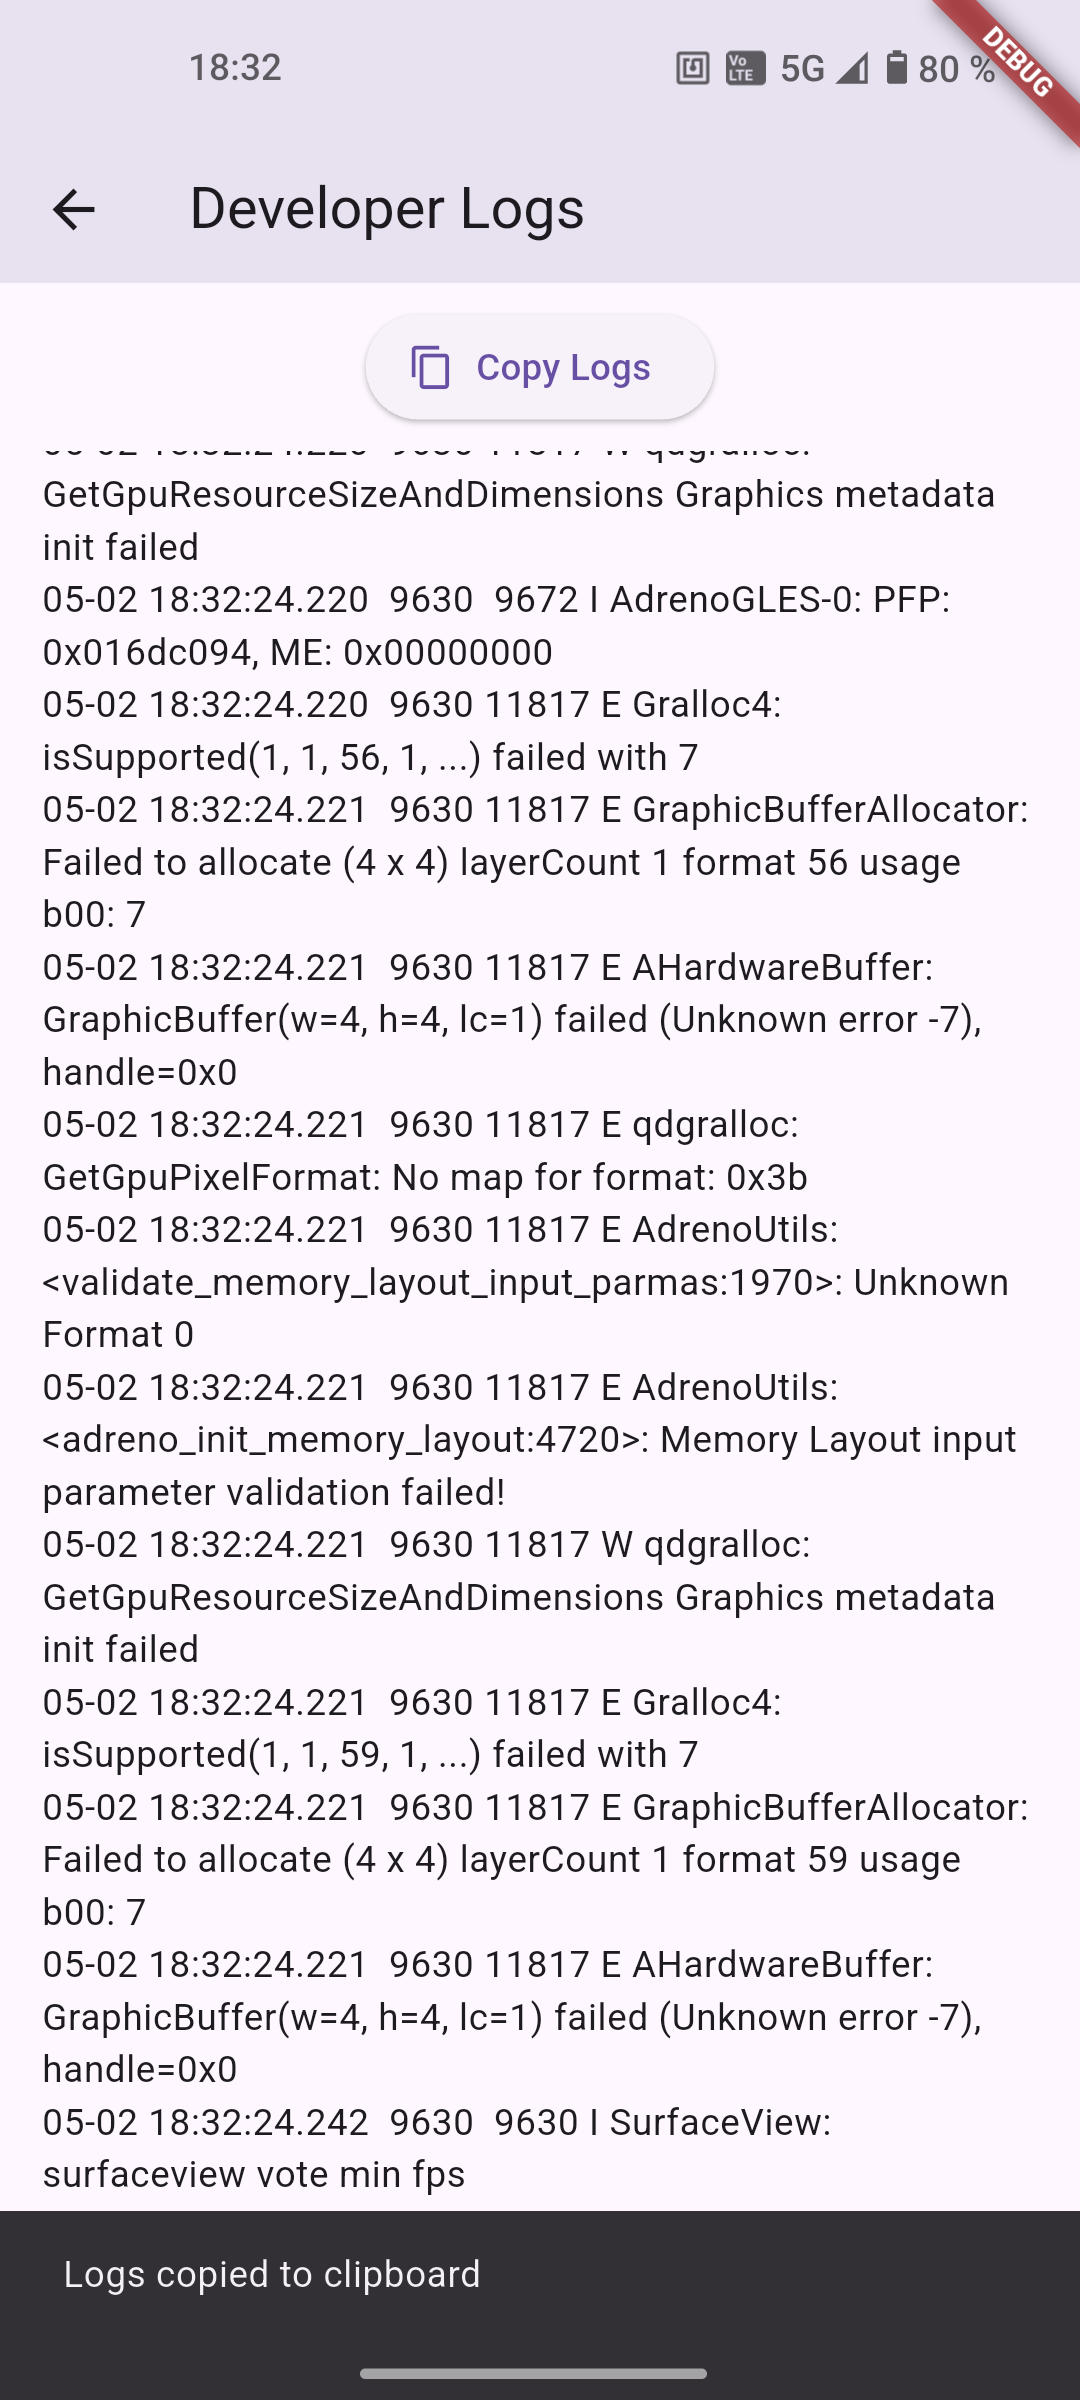
\includegraphics[width=\textwidth]{assets/developer_screen.png}
    \caption{Hidden developer screen}
    \label{fig:developer_screen}
  \end{figure}
\end{minipage}
\end{center}

\vspace{1em}

\begin{center}
\begin{minipage}{0.45\textwidth}
  \begin{figure}[H]
    \centering
    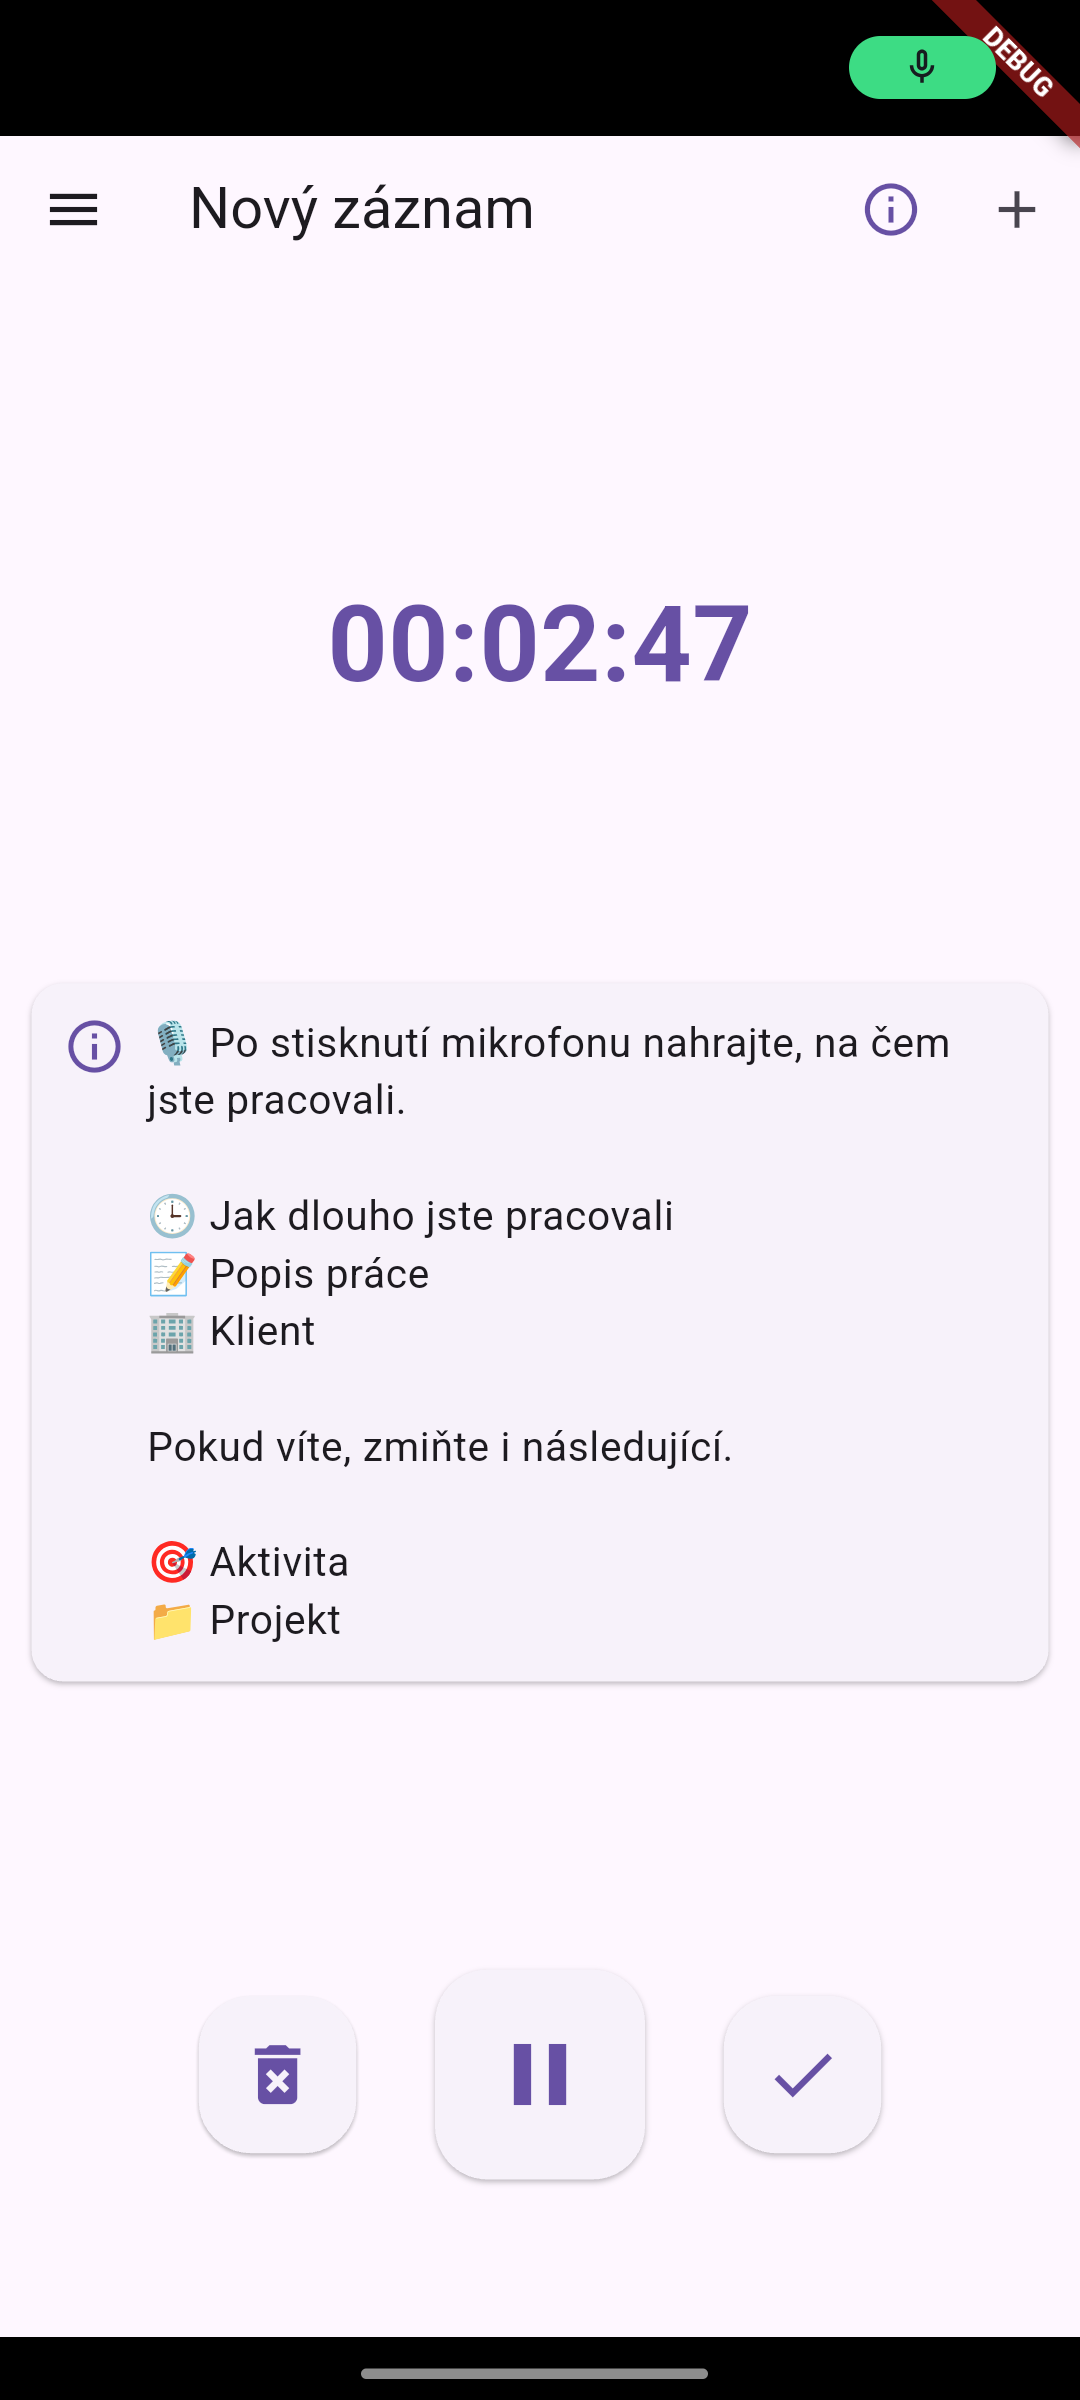
\includegraphics[width=\textwidth]{assets/recording_screen.png}
    \caption{Recording interface}
    \label{fig:recording_screen}
  \end{figure}
\end{minipage}
\hspace{0.05\textwidth}
\begin{minipage}{0.45\textwidth}
  \begin{figure}[H]
    \centering
    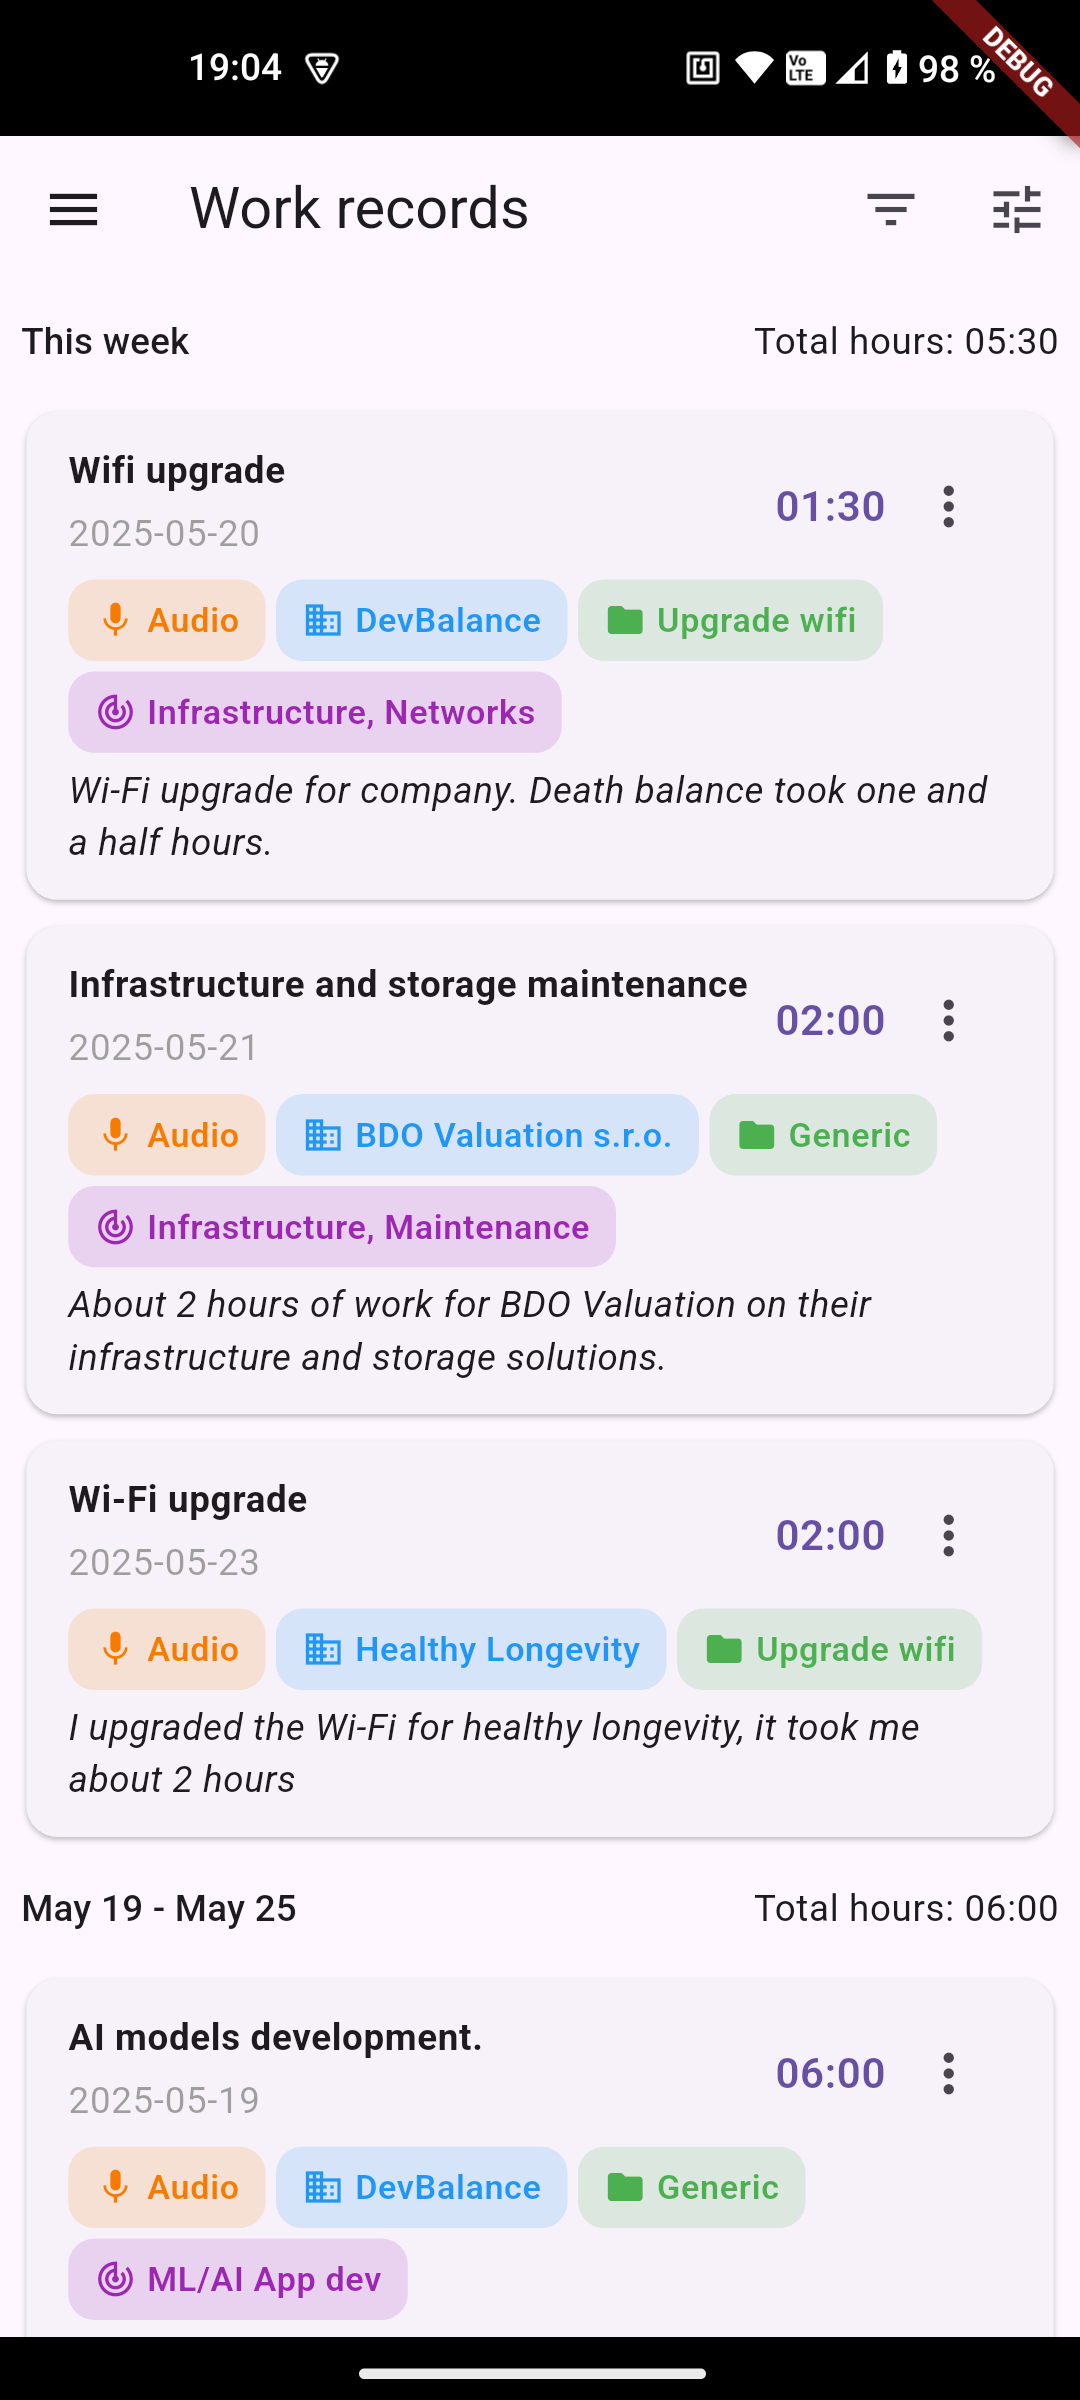
\includegraphics[width=\textwidth]{assets/records_screen.png}
    \caption{Overview of recorded entries}
    \label{fig:records_screen}
  \end{figure}
\end{minipage}
\end{center}

\vspace{1em}

\begin{center}
\begin{minipage}{0.45\textwidth}
  \begin{figure}[H]
    \centering
    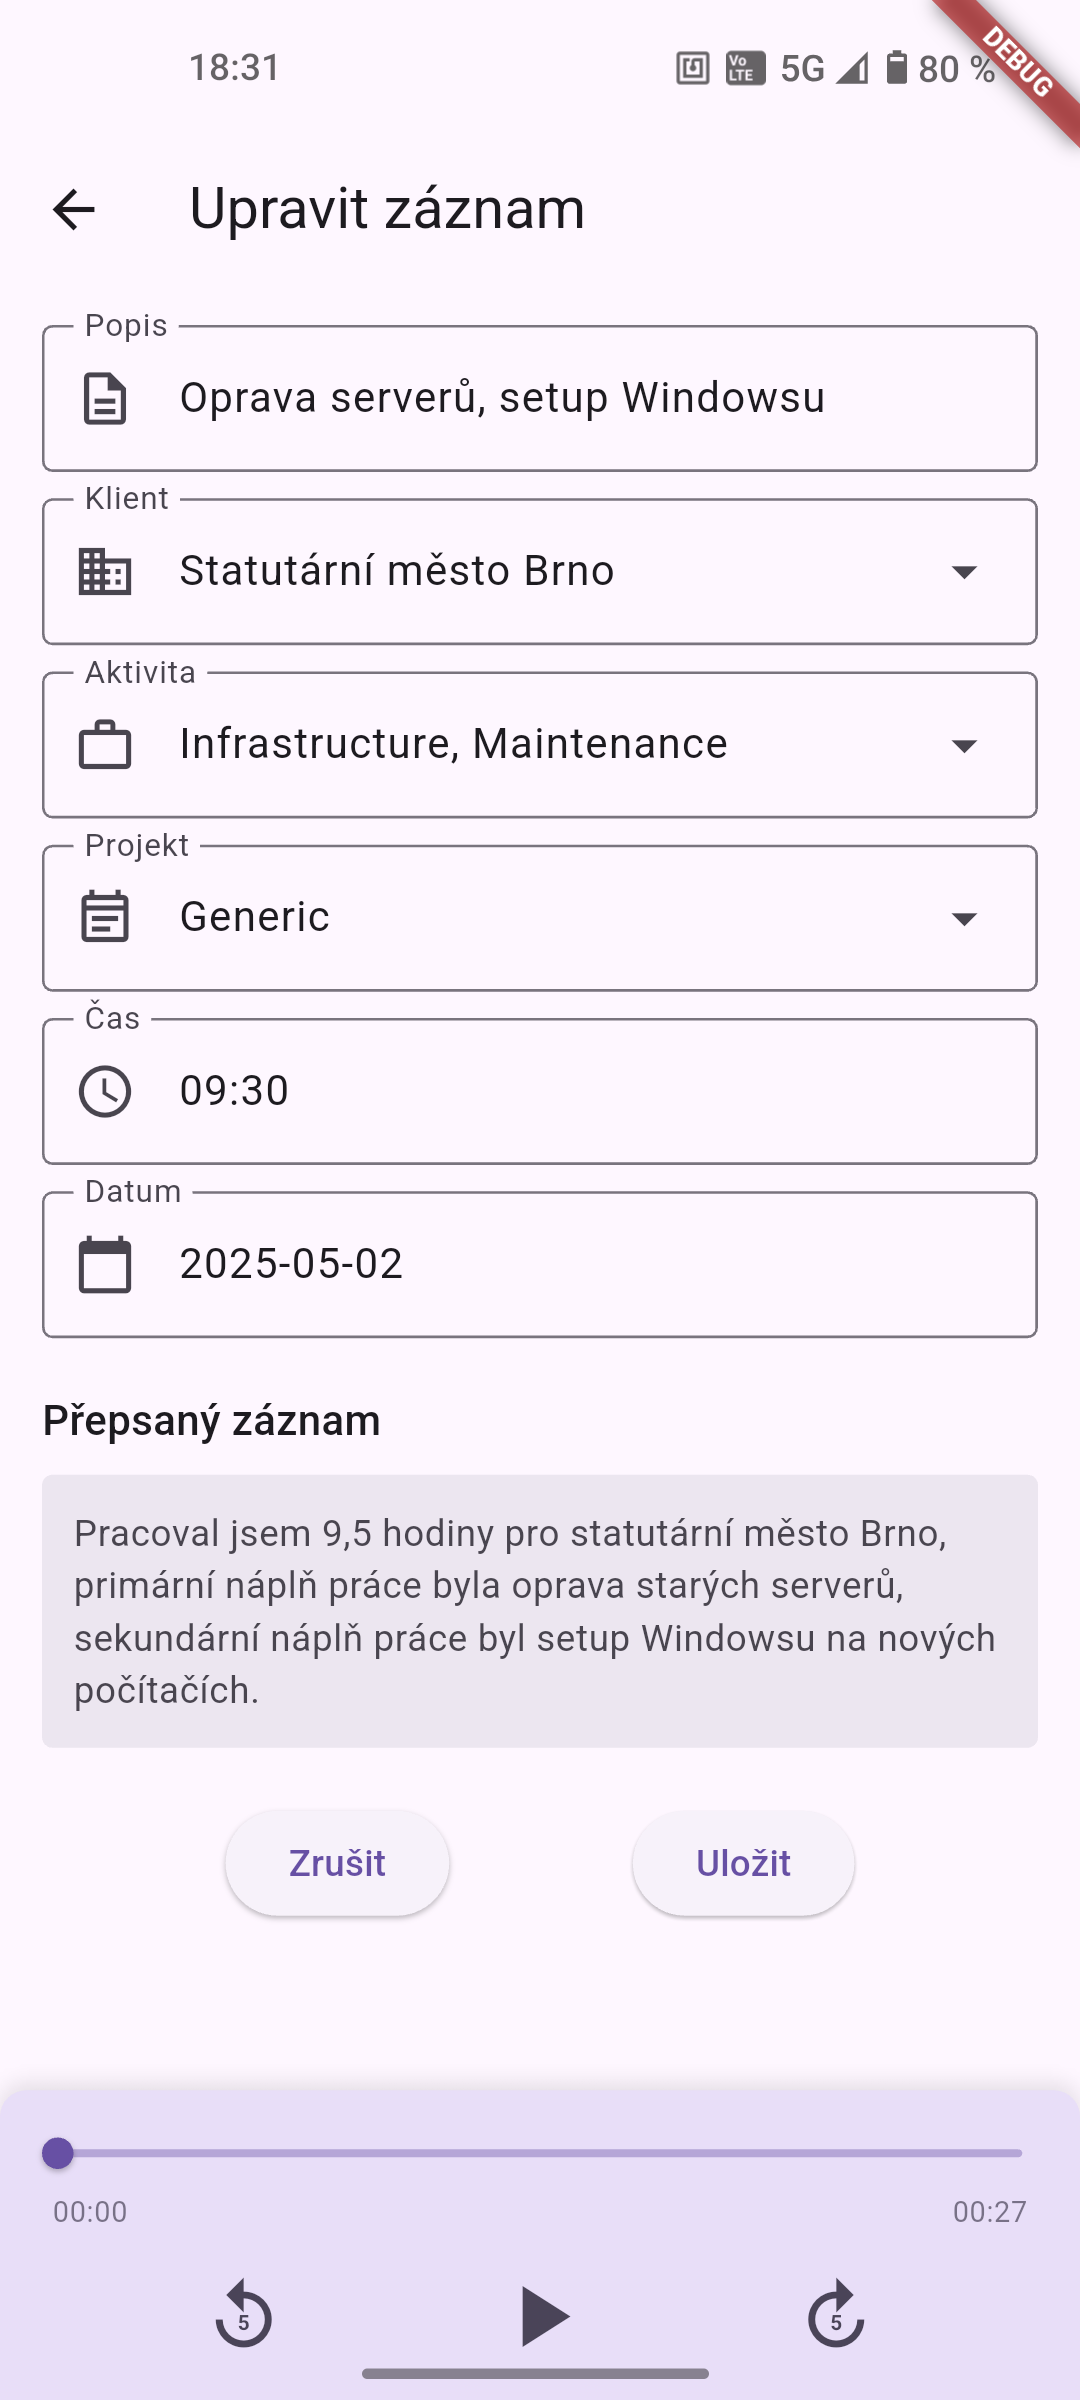
\includegraphics[width=\textwidth]{assets/edit_record.png}
    \caption{Editing a record}
    \label{fig:edit_record}
  \end{figure}
\end{minipage}
\hspace{0.05\textwidth}
\begin{minipage}{0.45\textwidth}
  \begin{figure}[H]
    \centering
    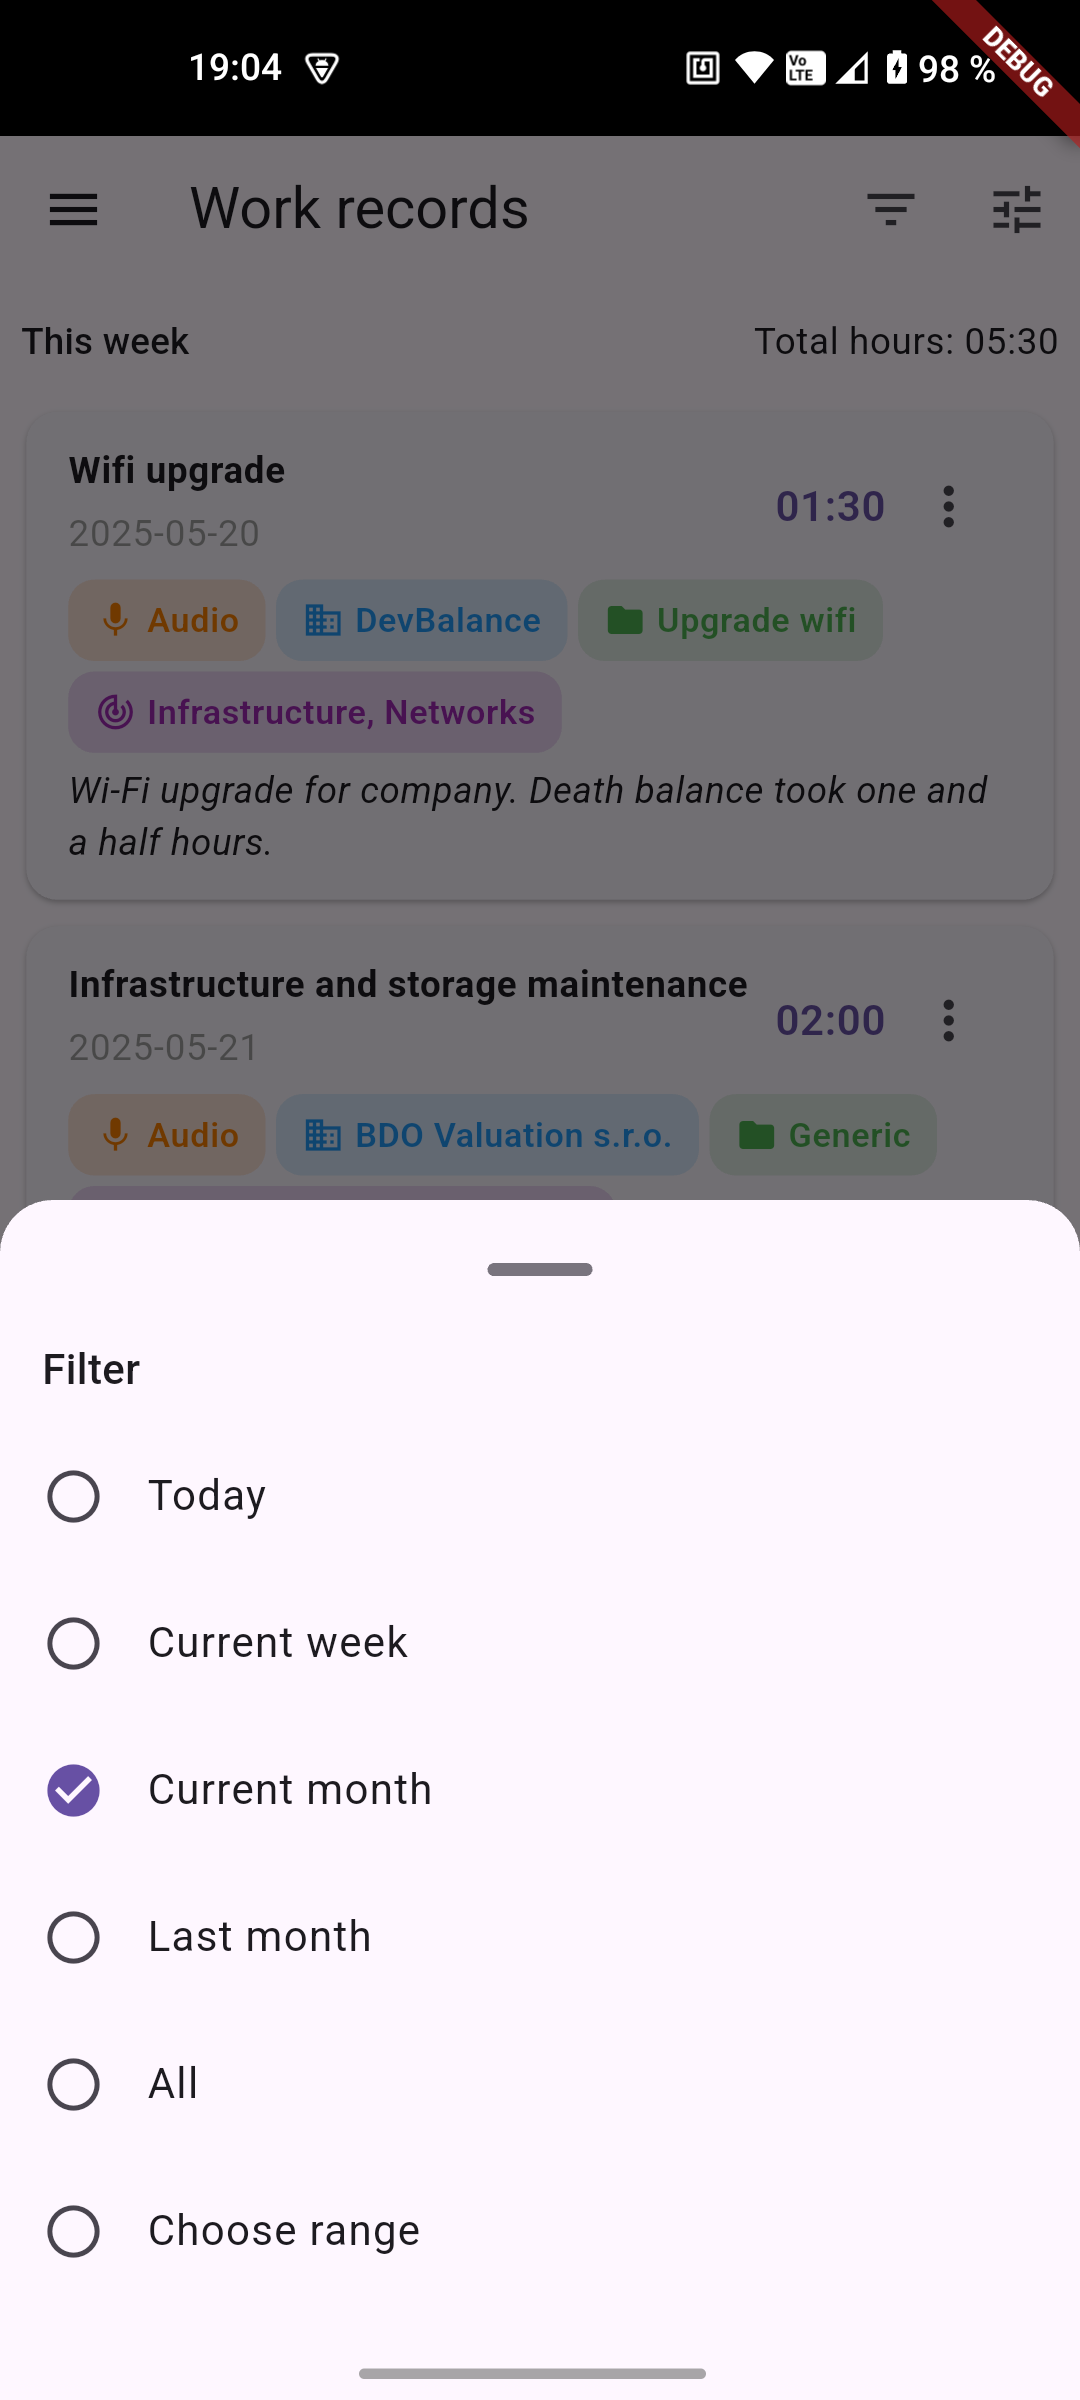
\includegraphics[width=\textwidth]{assets/filter_records_by.png}
    \caption{Filtering records by criteria}
    \label{fig:filter_records}
  \end{figure}
\end{minipage}
\end{center}

\vspace{1em}

\begin{center}
\begin{minipage}{0.45\textwidth}
  \begin{figure}[H]
    \centering
    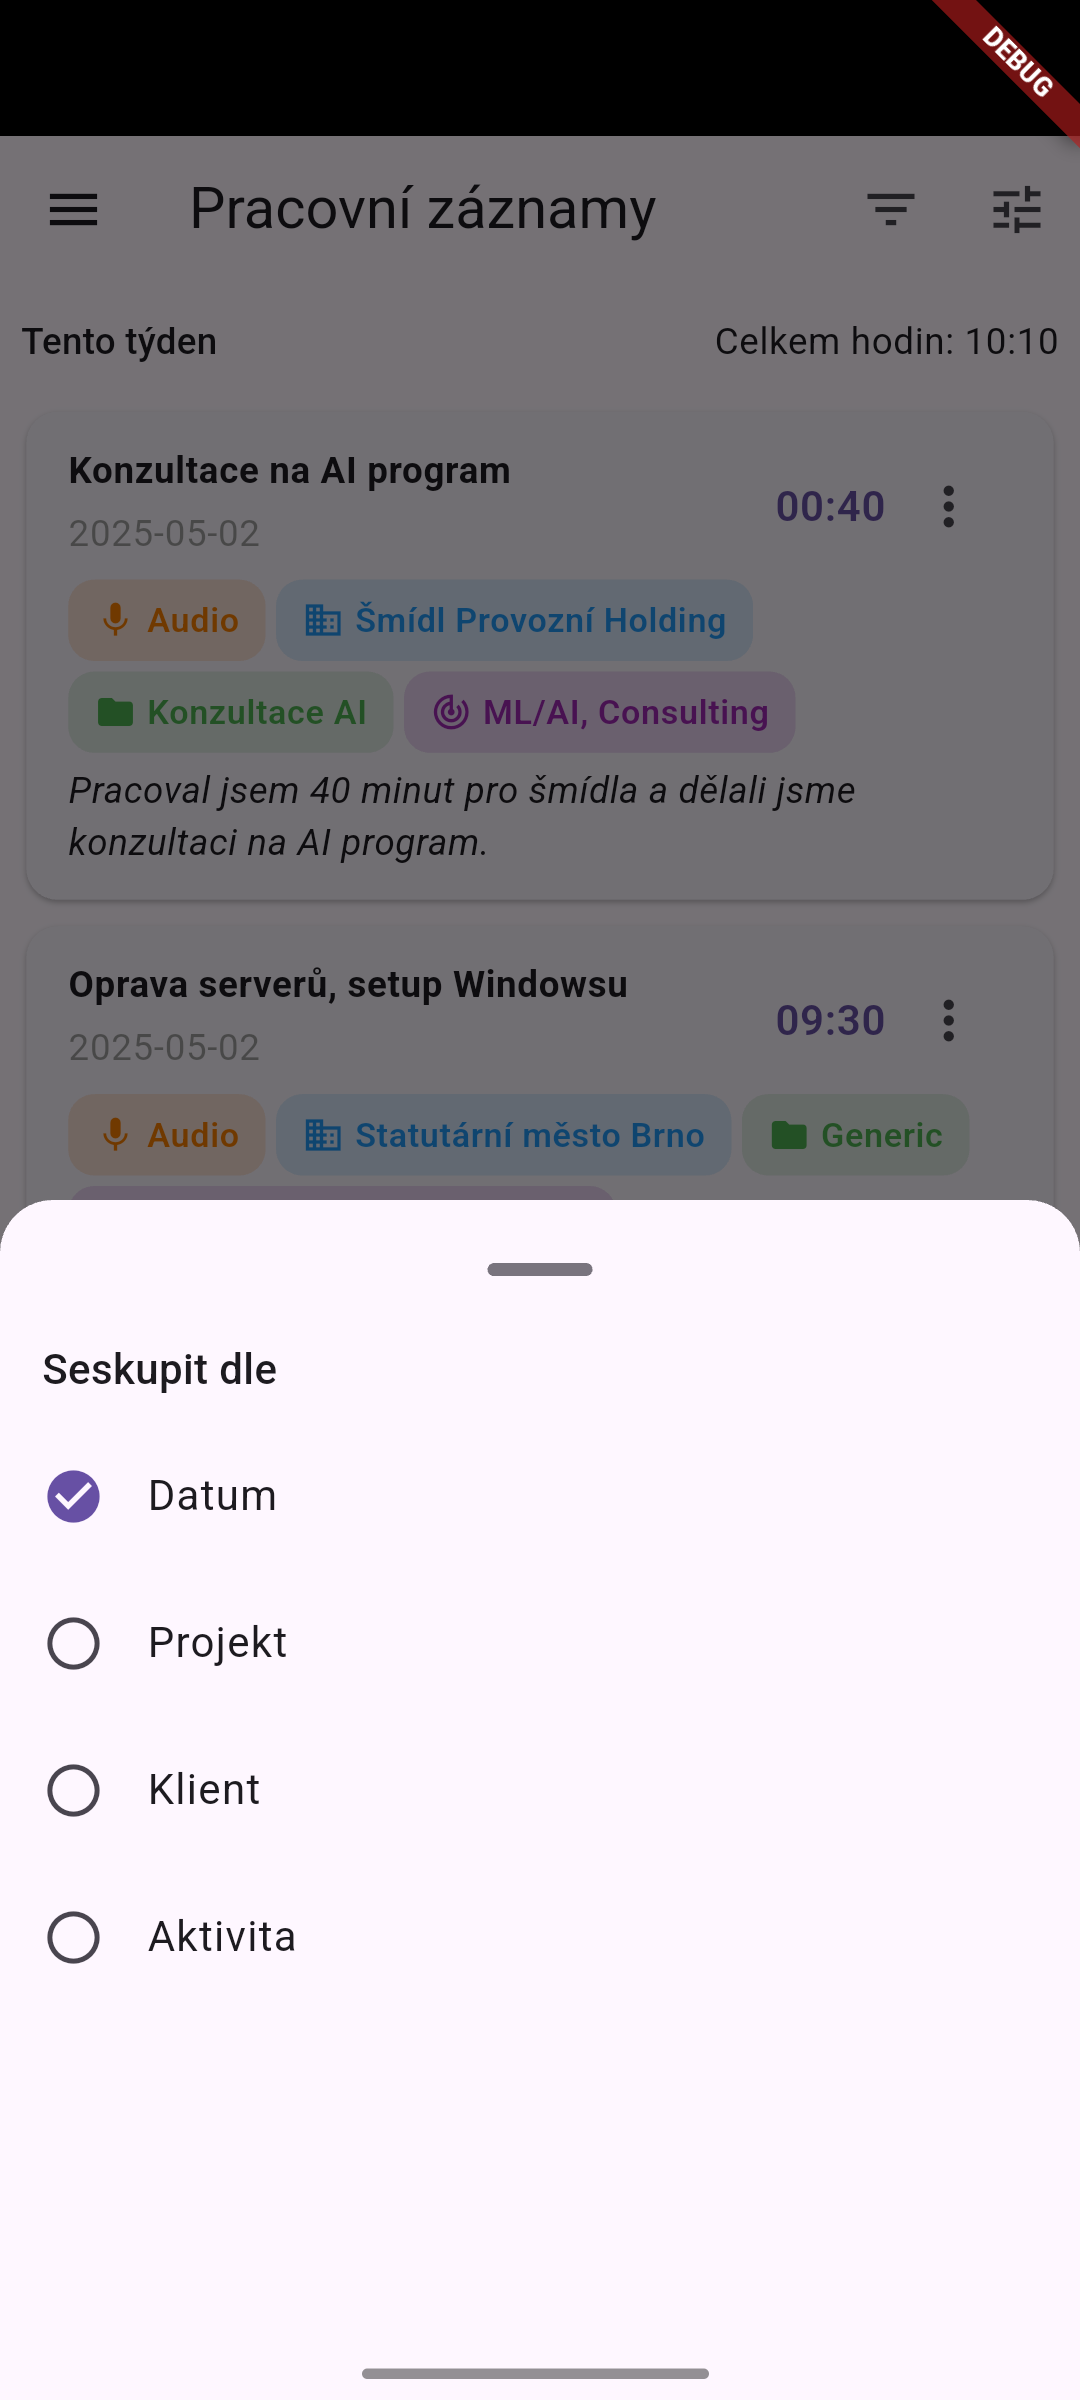
\includegraphics[width=\textwidth]{assets/group_records_by.png}
    \caption{Grouping records by attributes}
    \label{fig:group_records}
  \end{figure}
\end{minipage}
\hspace{0.05\textwidth}
\begin{minipage}{0.45\textwidth}
  \begin{figure}[H]
    \centering
    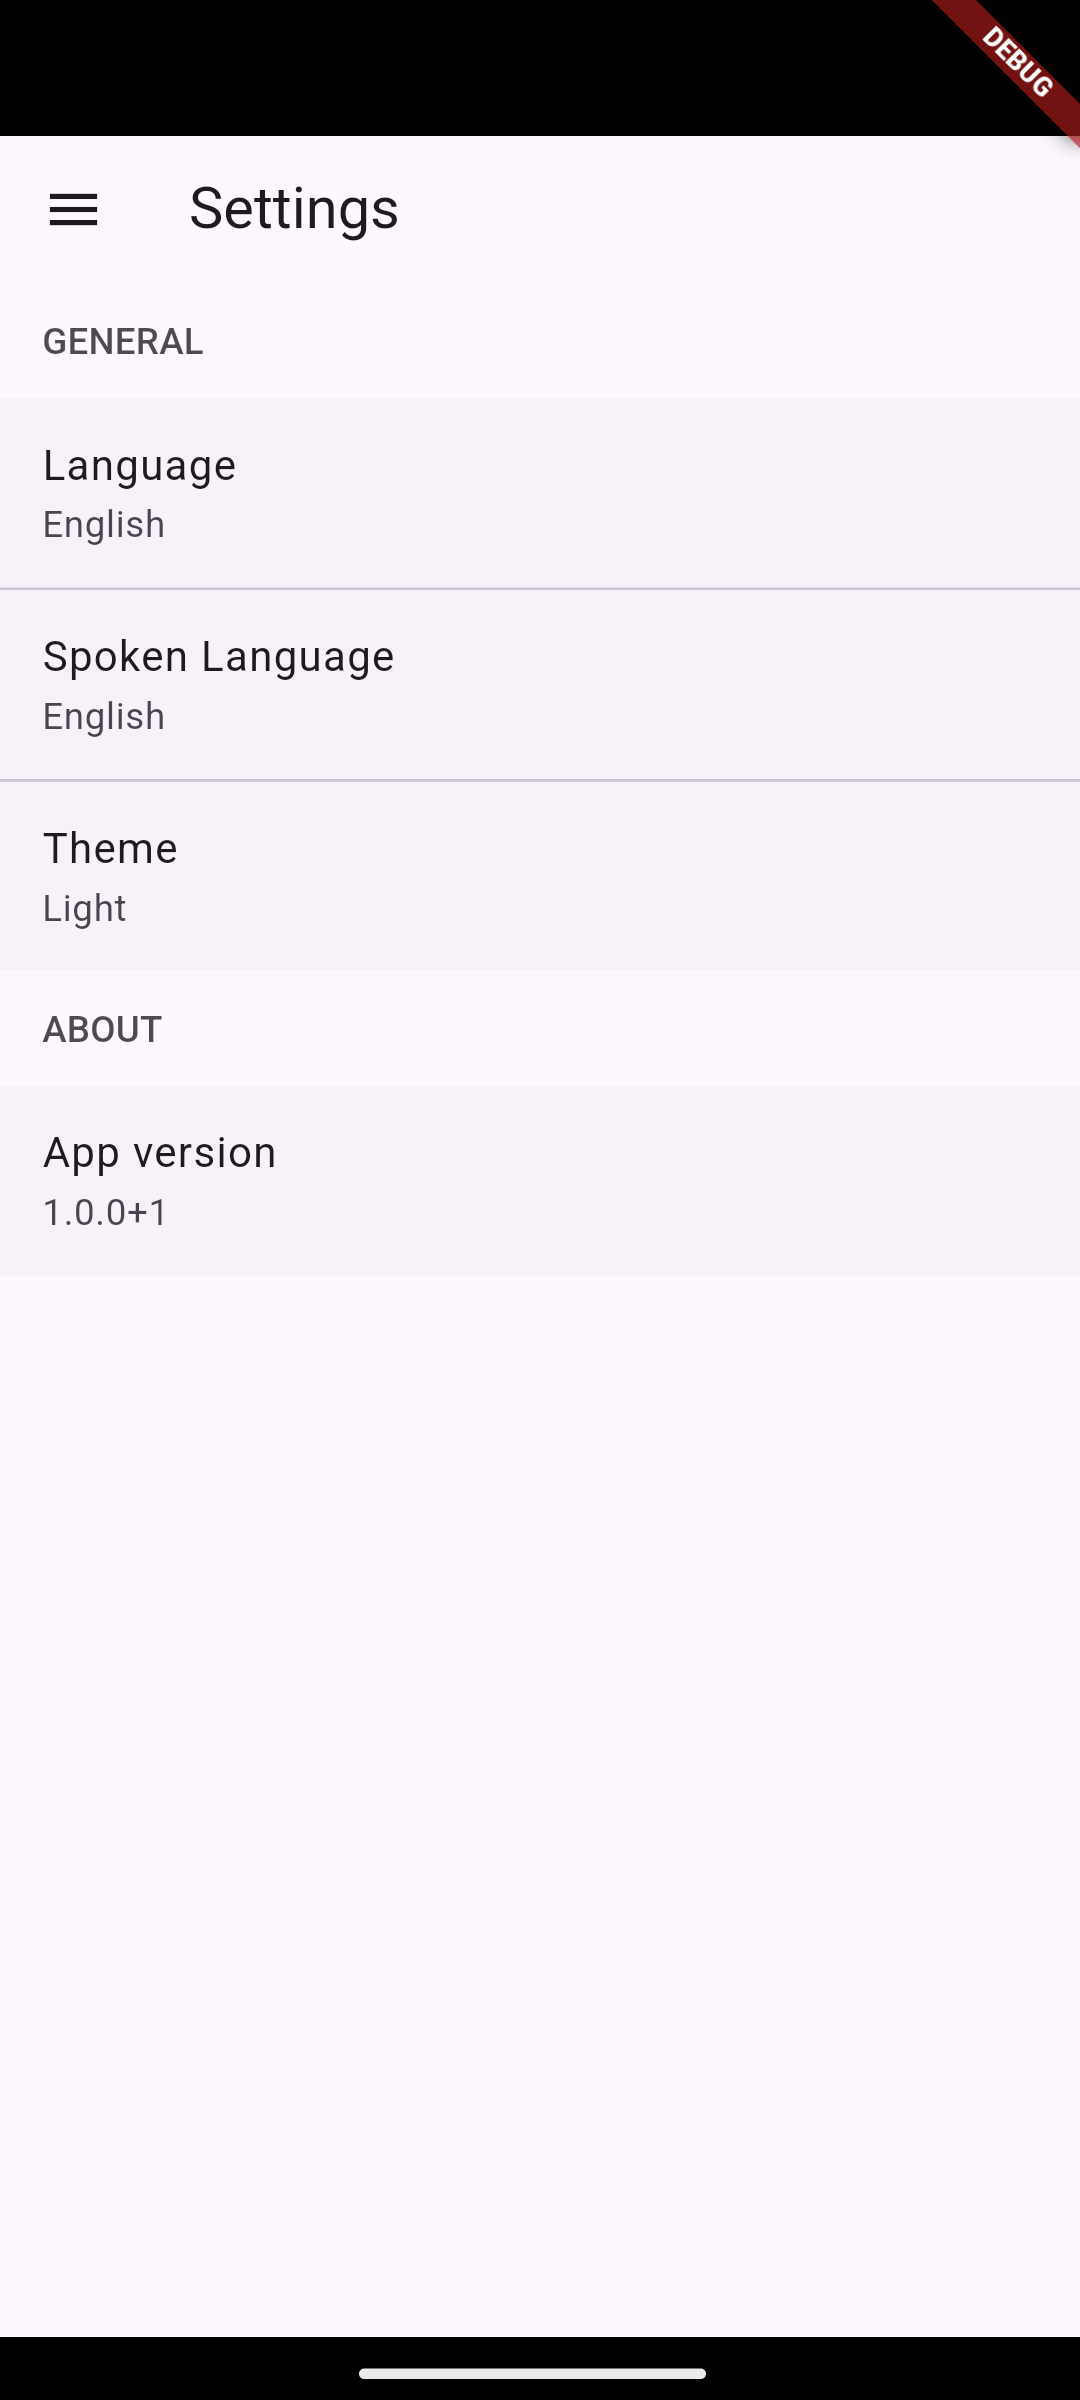
\includegraphics[width=\textwidth]{assets/settings_screen.png}
    \caption{Settings screen}
    \label{fig:settings_screen}
  \end{figure}
\end{minipage}
\end{center}


\end{document}
